\documentclass[12pt,a4paper]{article}

% ──────────────────────────── Packages ────────────────────────────
\usepackage[utf8]{inputenc}
\usepackage[T1]{fontenc}
\usepackage{lmodern}
\usepackage{microtype}
\usepackage{mathpazo}
\usepackage[scaled=0.92]{helvet}
\usepackage{eulervm}

\usepackage{graphicx}
\usepackage{amsmath,amssymb,amsfonts}
\usepackage{booktabs}
\usepackage{array}
\usepackage{float}
\usepackage{hyperref}
\usepackage{xcolor}
\usepackage{listings}
\usepackage{algorithm}
\usepackage{algpseudocode}
\usepackage{tikz}
\usetikzlibrary{shapes.geometric, arrows.meta, positioning, calc, fit, backgrounds, decorations.pathreplacing, chains, matrix}
\usepackage{pgfplots}
\pgfplotsset{compat=1.17}
\usepackage{subcaption}
\usepackage{multirow}
\usepackage{enumitem}
\usepackage{tabularx}
\usepackage{longtable}
\usepackage{setspace}
\usepackage{fancyhdr}
\usepackage{titlesec}
\usepackage{todonotes}
\usepackage[most]{tcolorbox}
\usepackage{colortbl}
% Reusable dashed equation/table box (defined after xcolor so headerblue is available)
\AtBeginDocument{%
  \tcbset{
    dashedbox/.style={
      enhanced, colback=white, colframe=white,
      borderline={0.8pt}{0pt}{headerblue, dashed},
      arc=6pt, boxrule=0pt,
      left=14pt, right=14pt, top=6pt, bottom=6pt
    }
  }%
}

% ──────────────────────────── Page Geometry ────────────────────────
\usepackage[
    top=2.5cm,
    bottom=2.5cm,
    left=1.8cm,
    right=1.8cm,
    headheight=14pt
]{geometry}

% ──────────────────────────── Colors ──────────────────────────────
\definecolor{marsred}{RGB}{150,40,20}
\definecolor{sandcolor}{RGB}{180,140,90}
\definecolor{deepblue}{RGB}{40,60,100}
\definecolor{codegreen}{RGB}{0,100,0}
\definecolor{boxgray}{RGB}{248,248,248}
\definecolor{headerblue}{RGB}{50,80,130}
\definecolor{accentorange}{RGB}{200,100,30}
\definecolor{softgreen}{RGB}{60,140,60}
\definecolor{softpurple}{RGB}{100,60,150}
\definecolor{softcyan}{RGB}{40,130,150}
\definecolor{lightblue}{RGB}{220,235,250}
\definecolor{lightorange}{RGB}{255,235,210}
\definecolor{lightred}{RGB}{255,220,220}
\definecolor{lightgreen}{RGB}{220,245,220}
\definecolor{lightgray}{RGB}{240,240,240}

% ──────────────────────────── Listings ────────────────────────────
\lstset{
    basicstyle=\ttfamily\small,
    keywordstyle=\color{deepblue}\bfseries,
    commentstyle=\color{codegreen},
    stringstyle=\color{marsred},
    frame=single,
    breaklines=true,
    captionpos=b,
    backgroundcolor=\color{boxgray},
    numbers=left,
    numberstyle=\tiny\color{gray},
    numbersep=5pt
}

% ──────────────────────────── Hyperref ────────────────────────────
\hypersetup{
    colorlinks=true,
    linkcolor=deepblue,
    citecolor=marsred,
    urlcolor=deepblue
}

% ──────────────────────────── Headers ─────────────────────────────
\pagestyle{fancy}
\fancyhf{}
\fancyhead[L]{\small\textit{Regolith Wheel Entrapment Recovery}}
\fancyhead[R]{\small\thepage}
\renewcommand{\headrulewidth}{0.4pt}

% ──────────────────────────── Spacing ─────────────────────────────
\setstretch{1.15}

% ──────────────── Placeholder command for images ──────────────────
% Use this for screenshots/photos to be added later
\newcommand{\imagePlaceholder}[3][]{%
    % #1 = optional width (default \textwidth)
    % #2 = height
    % #3 = caption text inside the box
    \begin{tikzpicture}
        \node[draw=gray!60, fill=lightgray, minimum width={\ifx&#1&\linewidth\else#1\fi},
              minimum height=#2, align=center, font=\small\itshape, text=gray!70,
              inner sep=10pt, rounded corners=2pt] {
            \parbox{0.8\linewidth}{\centering #3}
        };
    \end{tikzpicture}%
}

% ══════════════════════════════════════════════════════════════════
\begin{document}

% ──────────────────────────── Title Page ──────────────────────────
\begin{titlepage}
\centering
\vspace*{2cm}

{\Large\textsc{University of Dhaka}}\\[0.3em]
{\large\textsc{Department of Robotics and Mechatronics Engineering}}\\[2cm]

\rule{\textwidth}{1.5pt}\\[0.6cm]
{\LARGE\bfseries Adaptive Neural Control for Mars Rover\\[0.3em]
Wheel Entrapment Recovery in\\[0.3em]
Granular Terrain}\\[0.4cm]
\rule{\textwidth}{1.5pt}\\[1.5cm]

{\large\textit{A Research Project Report}}\\[2cm]

\begin{tabular}{rl}
\textbf{Authors:} & Meraj Hossain Promit \\
                   & Chandak Chakma \\[1em]
\textbf{Program:} & B.Sc. in Robotics and Mechatronics Engineering \\[0.5em]
\textbf{Supervisor:} & \textit{[Supervisor Name]} \\
\end{tabular}

\vfill
{\large April 2026}
\end{titlepage}

% ──────────────────────────── Abstract ────────────────────────────
\newpage
\begin{abstract}
\noindent
This report presents a reinforcement learning (RL) framework for autonomous recovery of Mars rovers from wheel entrapment in granular regolith. We leverage the Newton physics engine with Material Point Method (MPM)~\cite{sulsky1994particle} for high-fidelity granular soil simulation, Isaac Lab~\cite{isaaclab} for articulated robot simulation, and Proximal Policy Optimization (PPO)~\cite{schulman2017ppo} with recurrent GRU networks~\cite{cho2014gru} for policy training via the skrl library~\cite{skrl}. The system addresses the critical challenge of wheel entrapment faced by planetary exploration rovers, as exemplified by NASA's Spirit rover incident in 2009~\cite{arvidson2011spirit}, by training escape policies in a physically realistic simulation environment.

Our approach features a 29-dimensional proprioceptive observation space incorporating wheel velocities, slip ratios, IMU data, drive torques, and dual-sensor entrapment detection flags. The policy is trained across 64 parallel environments with curriculum learning that progressively deepens wheel sinkage from 8\,cm to 15\,cm. Preliminary results over 200,000 timesteps on an RTX 5070 Ti demonstrate an 80\% escape rate, mean forward velocity of 0.25\,m/s, and full curriculum completion. The trained policy exhibits emergent escape behaviors including rocking maneuvers and coordinated wheel--steering actions.

Future work includes scaling training to 2M+ timesteps, developing a CNN-GRU sinkage detection classifier, and deploying the trained policy on a Raspberry Pi 5 via ONNX Runtime for real-time inference on physical hardware.
\end{abstract}

% ──────────────────────────── TOC ─────────────────────────────────
\newpage
\tableofcontents

\newpage
\listoffigures
\listoftables

% ══════════════════════════════════════════════════════════════════
%                        1. INTRODUCTION
% ══════════════════════════════════════════════════════════════════
\newpage
\section{Introduction}

% ── Opening highlight box ──────────────────────────────────────────────────
\begin{tcolorbox}[
    enhanced, colback=white, colframe=headerblue,
    boxrule=0.8pt, arc=5pt,
    left=12pt, right=12pt, top=8pt, bottom=8pt
]
{\color{black!60} On May 1, 2009, NASA's Spirit rover drove into soft sulfate-rich soil and
never moved again. Eight months of recovery attempts, thousands of ground-based
tests, and 150 million kilometres of communication delay could not save it.
This project asks: \textbf{what if the rover could have saved itself?}}
\end{tcolorbox}

\vspace{8pt}

\subsection{Problem Statement}

Planetary exploration rovers operating on Mars and other celestial bodies~\cite{squyres2004mer,grotzinger2012msl,farley2020mars2020} face a critical operational challenge: \textbf{wheel entrapment in granular regolith}. When a rover's wheels sink into loose sand or soil, the vehicle loses mobility and may become permanently immobilized. This problem is particularly acute for several reasons:

\begin{itemize}[leftmargin=*, itemsep=3pt]
    \item \textbf{Rocker-bogie suspension}: While excellent for rough terrain, it distributes weight in ways that can cause individual wheels to sink disproportionately in soft soil.
    \item \textbf{Sandy and cratered terrain}: The Martian surface contains extensive dune fields, impact craters filled with fine regolith, and wind-blown sand deposits that present persistent mobility hazards.
    \item \textbf{Long communication delays}: With Earth--Mars one-way latencies of 4--24 minutes, real-time teleoperation for recovery is impractical, necessitating fully autonomous solutions.
    \item \textbf{Extended mission lifetimes}: As missions extend beyond planned durations, rovers inevitably encounter terrain types not anticipated during original mission planning.
\end{itemize}

\vspace{4pt}
Wheel entrapment is formally characterised by the simultaneous satisfaction of three conditions:

\begin{tcolorbox}[dashedbox]
\begin{equation}
    f_{\text{ent}} = 1 \;\iff\;
    \begin{cases}
        |v_x| < 0.15\;\text{m/s} & \text{(near-zero forward velocity)} \\[4pt]
        \bar{\sigma}_{\text{slip}} > 0.4 & \text{(high mean wheel slip)} \\[4pt]
        d_{\text{sinkage}} > 0 & \text{(positive wheel sinkage)}
    \end{cases}
    \label{eq:entrapment_definition}
\end{equation}
\end{tcolorbox}

\noindent where $v_x$ is the body-frame forward velocity, $\bar{\sigma}_{\text{slip}} = \frac{1}{6}\sum_i \sigma_i$ is the mean slip ratio across all six drive wheels, and $d_{\text{sinkage}}$ is the wheel sinkage depth into the granular medium. All three conditions must hold for at least \textbf{15 consecutive steps} ($0.6\,\text{s}$) before the entrapment flag $f_{\text{ent}}$ is raised.

\subsection{Problem Definition}

The entrapment recovery problem is formulated as a \textbf{partially observable Markov decision process (POMDP)}. At each timestep $t$, the rover receives a proprioceptive observation $\mathbf{o}_t \in \mathbb{R}^{29}$ and must select an action $\mathbf{a}_t \in \mathbb{R}^{10}$ to maximise the expected discounted return:
\begin{tcolorbox}[dashedbox]
\begin{equation}
    J(\pi_\theta) = \mathbb{E}_{\tau \sim \pi_\theta}
    \left[ \sum_{t=0}^{T} \gamma^t\, R(\mathbf{s}_t, \mathbf{a}_t) \right], \qquad \gamma = 0.99
    \label{eq:objective}
\end{equation}
\end{tcolorbox}

The shaped reward $R$ is the sum of seven terms — three incentives and four penalties — designed to reward escape while discouraging dangerous manoeuvres:

\begin{tcolorbox}[dashedbox]
\begin{equation}
    R_t \;=\; \underbrace{r_{\text{progress}} + r_{\text{escape}} + r_{\text{rocking}}}_{\text{incentives}}
          \;-\; \underbrace{p_{\text{slip}} + p_{\text{tilt}} + p_{\text{smooth}} + p_{\text{abnormal}}}_{\text{penalties}}
    \label{eq:reward_total}
\end{equation}
\end{tcolorbox}

\vspace{6pt}

\begin{tcolorbox}[dashedbox, left=0pt, right=0pt, top=4pt, bottom=4pt]
\begin{table}[H]
\centering
\small
\setlength{\tabcolsep}{8pt}
\renewcommand{\arraystretch}{1.4}
\begin{tabularx}{\linewidth}{llX}
\toprule
\rowcolor{lightblue}
\textbf{Term} & \textbf{Weight} & \textbf{Formula \& Description} \\
\midrule
\multicolumn{3}{l}{\textbf{Incentives}} \\
\midrule
$r_{\text{progress}}$ & $+1.5$  & $v_x \cdot \Delta t \cdot (1 - f_{\text{ent}})$ \quad — forward velocity reward, suppressed when trapped so rocking takes over \\
$r_{\text{escape}}$   & $+20.0$ & Sparse milestones at 0.5\,m ($\times0.2$), 1.0\,m ($\times0.4$), 1.5\,m ($\times1.0$) scaled by $\tau_{\text{time}}$; plus dense shaping $0.5\,d\,\Delta t$ per step \\
$r_{\text{rocking}}$  & $+2.0$  & $\Delta v_x \cdot f_{\text{ent}} \cdot \Delta t$ \quad — rewards velocity change during entrapment to encourage active rocking manoeuvres \\
\midrule
\multicolumn{3}{l}{\textbf{Penalties}} \\
\midrule
$p_{\text{slip}}$     & $0.5$  & $\bar{\sigma}_{\text{slip}} \cdot (1 - f_{\text{ent}}) \cdot \Delta t$ \quad — penalises excessive wheel slip during normal driving \\
$p_{\text{tilt}}$     & $0.3$  & $\|\boldsymbol{\omega}_{xy}\|_2 \cdot \Delta t$ \quad — penalises roll/pitch angular velocity to maintain rover stability \\
$p_{\text{smooth}}$   & $0.05$ & $\|\mathbf{a}_t - \mathbf{a}_{t-1}\|_2 \cdot \Delta t$ \quad — penalises jerky action changes to encourage smooth control \\
$p_{\text{abnormal}}$ & $0.3$  & $(-v_x)^{+} \cdot f_{\text{anomaly}} \cdot (1 - f_{\text{ent}}) \cdot \Delta t$ \quad — penalises backward motion under torque anomaly when not trapped \\
\bottomrule
\multicolumn{3}{l}{\footnotesize $f_{\text{ent}}$: entrapment flag;\enspace $f_{\text{anomaly}}$: torque anomaly flag;\enspace $d$: distance from spawn;\enspace $\Delta t = 0.04\,\text{s}$}
\end{tabularx}
\caption{Reward function v4 used during PPO training. The escape bonus (weight 20) dominates during entrapment, while the rocking bonus encourages active self-extraction. Compared to Bi \& Ding (2026)~\cite{bi2026escape}, who use GAIL-fused~\cite{ho2016gail} rewards ($R = 0.9R_H + 0.1R_D$) with expert demonstrations, our reward is fully handcrafted and designed for 6-DOF steering under Martian gravity without requiring any expert data.}
\label{tab:reward_function}
\end{table}
\end{tcolorbox}

The partial observability arises because the rover cannot directly sense the depth of sinkage per wheel, the local terrain composition, or its position relative to the entrapment zone boundary. This motivates a \textbf{recurrent policy} based on the Gated Recurrent Unit (GRU)~\cite{cho2014gru} that maintains a hidden state $\mathbf{h}_t$ to implicitly estimate these unobserved variables from the history of observations. GRUs are a lightweight alternative to LSTMs~\cite{hochreiter1997lstm} that achieve comparable performance on temporal sequence modeling with fewer parameters.

\subsection{Motivation: The Spirit Rover Incident (2009)}

The most prominent example of wheel entrapment in planetary exploration occurred on May 1, 2009, when NASA's Mars Exploration Rover \textit{Spirit} became embedded in soft sulfate-rich regolith at a site named ``Troy'' near the western edge of Home Plate in Gusev Crater~\cite{arvidson2011spirit,squyres2004mer}. Figure~\ref{fig:spirit_timeline} illustrates the timeline of this critical incident.

\begin{figure}[H]
\centering
% RESIZEBOX IS THE FIX ---
% This forces the diagram to fit exactly within the text width of your document.
\resizebox{\textwidth}{!}{%
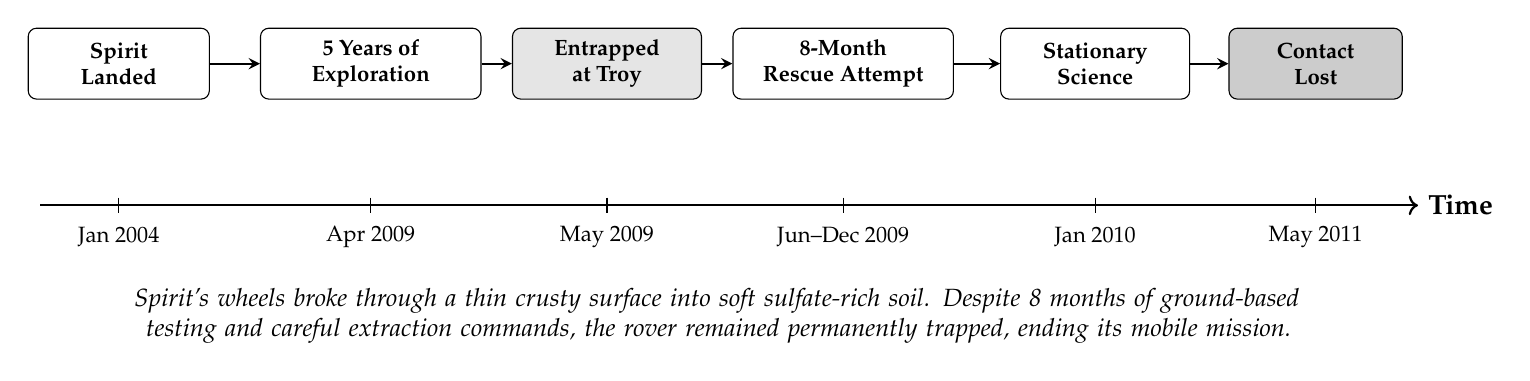
\begin{tikzpicture}[
    box/.style={rectangle, rounded corners=3pt, draw=black, fill=white,
                minimum height=0.9cm, align=center, font=\footnotesize\bfseries},
    arrow/.style={->, >=stealth, thick}
]
    % Place boxes with explicit spacing
    \node[box, minimum width=2.3cm] (b1) at (0,0) {Spirit\\Landed};
    \node[box, minimum width=2.8cm] (b2) at (3.2,0) {5 Years of\\Exploration};
    \node[box, minimum width=2.4cm, fill=gray!20] (b3) at (6.2,0) {Entrapped\\at Troy};
    \node[box, minimum width=2.8cm] (b4) at (9.2,0) {8-Month\\Rescue Attempt};
    \node[box, minimum width=2.4cm] (b5) at (12.4,0) {Stationary\\Science};
    \node[box, minimum width=2.2cm, fill=gray!40] (b6) at (15.2,0) {Contact\\Lost};

    % Draw unidirectional arrows (right only)
    \draw[arrow] (b1) -- (b2);
    \draw[arrow] (b2) -- (b3);
    \draw[arrow] (b3) -- (b4);
    \draw[arrow] (b4) -- (b5);
    \draw[arrow] (b5) -- (b6);

    % Timeline
    \draw[->, thick] (-1,-1.8) -- (16.5,-1.8) node[right] {\textbf{Time}};

    % Timeline markers
    \foreach \x/\lbl in {0/Jan 2004, 3.2/Apr 2009, 6.2/May 2009,
                          9.2/Jun--Dec 2009, 12.4/Jan 2010, 15.2/May 2011} {
        \draw (\x,-1.7) -- (\x,-1.9);
        \node[font=\footnotesize] at (\x,-2.2) {\lbl};
    }

    % Description text
    \node[text width=15cm, align=center, font=\small\itshape] at (7.6,-3.2) {
        Spirit's wheels broke through a thin crusty surface into soft sulfate-rich soil.
        Despite 8 months of ground-based testing and careful extraction commands,
        the rover remained permanently trapped, ending its mobile mission.
    };
\end{tikzpicture}%
}
\caption{Timeline of the Spirit Rover entrapment incident. After 5 years of successful exploration, Spirit became permanently immobilized in soft regolith, motivating autonomous entrapment recovery research.}
\label{fig:spirit_timeline}
\end{figure}

Key lessons from the Spirit incident that inform this research:
\begin{enumerate}
    \item \textbf{Detection was delayed}: Spirit had driven partway into the soft soil before operators recognized the hazard, as slip ratio was not monitored in real-time.
    \item \textbf{Recovery required months}: The 8-month extraction campaign involved extensive Earth-based testing on rover replicas, constrained by communication delays.
    \item \textbf{Autonomous response was absent}: Spirit had no onboard capability to detect or respond to entrapment autonomously.
    \item \textbf{Granular physics are critical}: The behavior of the sulfate-rich soil was poorly understood, leading to extraction commands that inadvertently worsened the entrapment.
\end{enumerate}

\newpage
\subsection{Objectives}

This research aims to develop a complete autonomous entrapment detection and recovery system for Mars rovers. The five specific objectives are:

\tcbset{
    objbox/.style={
        enhanced,
        colback=white,
        colframe=headerblue,
        boxrule=0.8pt,
        arc=4pt,
        left=10pt, right=8pt, top=5pt, bottom=5pt,
        fonttitle=\small\bfseries,
        coltitle=black,
        attach title to upper,
        title after break={},
    }
}

\vspace{6pt}
\begin{tcolorbox}[objbox, colframe=headerblue, title={1.\enspace Realistic Simulation\enspace---\enspace}]
Build a high-fidelity simulation environment coupling granular material physics (Newton MPM)
with articulated rover dynamics (Isaac Lab) under Martian gravity ($3.72\,\text{m/s}^2$),
enabling realistic wheel--soil interaction for RL training.
\end{tcolorbox}

\vspace{4pt}
\begin{tcolorbox}[objbox, colframe=headerblue, title={2.\enspace Entrapment Detection\enspace---\enspace}]
Develop a dual-sensor detection scheme combining slip-ratio monitoring and drive-torque
anomaly detection for robust, real-time entrapment classification without external
sensing or GPS.
\end{tcolorbox}

\vspace{4pt}
\begin{tcolorbox}[objbox, colframe=headerblue, title={3.\enspace Recovery Policy\enspace---\enspace}]
Train a recurrent RL policy (PPO + GRU) that autonomously discovers and executes
effective escape manoeuvres — including rocking, steering pivots, and differential
drive — from varying degrees of wheel sinkage (6–12\,cm curriculum).
\end{tcolorbox}

\vspace{4pt}
\begin{tcolorbox}[objbox, colframe=headerblue, title={4.\enspace Curriculum Learning\enspace---\enspace}]
Implement progressive difficulty scheduling that begins with shallow sinkage and
gradually increases entrapment severity, enabling the policy to learn robust escape
strategies that generalise across terrain conditions.
\end{tcolorbox}

\vspace{4pt}
\begin{tcolorbox}[objbox, colframe=headerblue, title={5.\enspace Sim-to-Real Transfer\enspace---\enspace}]
Establish a complete deployment pipeline — domain randomisation during training,
ONNX export of the trained GRU policy, and real-time inference on a Raspberry Pi 5
— bridging the simulation--reality gap for onboard autonomous operation.
\end{tcolorbox}
\vspace{6pt}


% ══════════════════════════════════════════════════════════════════
%                       2. RELATED WORK
% ══════════════════════════════════════════════════════════════════
\newpage
\section{Related Work}

This section reviews prior work in three key areas: (1) wheeled robot entrapment and escape strategies, (2) granular media simulation for robotics, and (3) reinforcement learning for locomotion and recovery.

% ─────── 2.1 ──────────────────────────────────────────────────────
\subsection{Escape Strategies for Wheeled Robots}

\subsubsection{Bi and Ding (2026): DRL-Based Escape for Skid-Steered Mobile Robots}

Bi and Ding~\cite{bi2026escape} presented a deep reinforcement learning framework for escape and path point tracking of skid-steered mobile robots (SSMRs) under undulating terrain conditions in outdoor orchards. Their work is the most directly relevant to ours.

\paragraph{Description.} The authors developed a two-phase system: (1)~an abnormal state detection module using motor torque analysis, and (2)~a DRL-based escape policy using PPO with LSTM networks~\cite{hochreiter1997lstm}. Their key innovation is a \textit{reward fusion} strategy combining handcrafted rewards with GAIL-derived~\cite{ho2016gail} (Generative Adversarial Imitation Learning) discriminator rewards: $R = 0.9 R_H + 0.1 R_D$, where $R_H$ includes path tracking, abnormal action, and conditional rewards, and $R_D$ comes from a discriminator trained on expert demonstrations. The system was trained for 4 million timesteps in a Unity simulation environment with extensive domain randomization (20+ parameters, see their Table 9) and validated in real-world outdoor orchard conditions, achieving 90\% escape success rate in both simulation and field tests.

Their observation space comprised 30 dimensions organized as $\mathbf{s} = \{\mathbf{s}_{\text{motor}},\allowbreak\ \mathbf{s}_{\text{motion}},\allowbreak\ \mathbf{s}_{\text{position}},\allowbreak\ s_{\text{abnormal}}\}$: 16D motor data (set speed, current speed, current torque, average torque $\times$ 4 motors), 7D motion state (quaternion attitude + angular velocity), 2D position (distance and angle to target), and 1D anomaly flag. The action space is 2D: left and right wheel velocities $\mathbf{a} = [\omega_l, \omega_r]$.

\paragraph{Strengths.}
\begin{itemize}
    \item Achieved 90\% escape success rate in both simulation and real-world tests, demonstrating strong sim-to-real transfer via domain randomization.
    \item LSTM-based temporal modeling captures the sequential nature of entrapment dynamics, enabling memory-dependent escape strategies.
    \item GAIL reward fusion ($R = 0.9R_H + 0.1R_D$) combines human intuition with learned reward shaping, producing smoother and more natural escape trajectories compared to pure handcrafted or pure imitation approaches.
    \item Comprehensive anomaly detection based on motor torque threshold (Eq.~10 in their paper): $\frac{1}{c_t}\sum_{n=t-c_t}^{t}\frac{|^iT_n|}{T_N} > T_{\text{thread}}$ with $T_{\text{thread}} = 0.95$.
    \item Validated on real outdoor terrain (orchards) with undulating surfaces using UWB positioning.
\end{itemize}

\paragraph{Weaknesses.}
\begin{itemize}
    \item Limited to 4-wheel skid-steered platforms; does not address the more complex kinematics of 6-wheel rocker-bogie suspension systems used in Mars rovers (Curiosity, Perseverance).
    \item Uses rigid terrain simulation (Unity) and does not model granular soil mechanics (particle flow, sinkage dynamics, bulldozing resistance) that are critical for planetary regolith interaction.
    \item Tested under Earth gravity ($9.81\,\text{m/s}^2$), not Mars gravity ($3.72\,\text{m/s}^2$), which significantly affects soil--wheel traction and sinkage behavior.
    \item Requires expert demonstrations for GAIL training, which may not be available for novel Mars terrain conditions.
    \item Two-dimensional action space ($\omega_l, \omega_r$) does not leverage independent steering joints for more sophisticated escape maneuvers.
    \item Entrapment is caused by tire lift-off on undulating terrain, not by granular sinkage, which is a fundamentally different failure mode.
\end{itemize}


\subsubsection{Inotsume et al. (2020): Slip Prediction for Planetary Rovers}

\paragraph{Description.} Inotsume et al.~\cite{inotsume2020} investigated real-time slip prediction for planetary rovers using proprioceptive sensing and terrain parameter estimation. A Kalman filter fuses motor current, wheel sinkage estimates, and terrain slope to predict slip ratio based on Bekker--Wong terramechanics theory.

\paragraph{Strengths.}
\begin{itemize}
    \item Principled physics-based approach grounded in terramechanics theory; provides interpretable terrain parameter estimates.
    \item Runs in real-time on embedded hardware with low computational requirements.
    \item Directly applicable to Mars rover missions with existing sensor suites.
\end{itemize}

\paragraph{Weaknesses.}
\begin{itemize}
    \item Focuses on slip prediction only; does not address active recovery from entrapment.
    \item Requires careful calibration for each terrain type, limiting generalization to unknown Martian soils.
    \item Simplified Bekker--Wong model may not capture complex particle--wheel coupling during deep sinkage.
\end{itemize}


\subsubsection{Ding et al. (2011): Wheel--Terrain Interaction Modeling}

\paragraph{Description.} Ding et al.~\cite{ding2011} presented a comprehensive wheel--soil interaction model for planetary rovers, deriving analytical expressions for drawbar pull, rolling resistance, and sinkage as functions of wheel geometry, soil parameters (cohesion, internal friction angle, shear deformation modulus), and slip ratio. The model accounts for multi-pass effects where trailing wheels encounter pre-compacted soil.

\paragraph{Strengths.}
\begin{itemize}
    \item Rigorous analytical framework validated experimentally with single-wheel testbed data.
    \item Accounts for multi-wheel interactions and soil compaction by preceding wheels.
\end{itemize}

\paragraph{Weaknesses.}
\begin{itemize}
    \item Steady-state analysis only; does not capture transient dynamics during entrapment onset or recovery.
    \item Assumes homogeneous soil properties, unrealistic for heterogeneous Martian terrain.
    \item Does not address control strategies for escape from entrapment.
\end{itemize}


\subsubsection{Jain et al. (2019): RL for Planetary Rover Locomotion}

\paragraph{Description.} Jain et al.~\cite{jain2019} applied DQN for adaptive locomotion of planetary rovers, learning to select discrete gaits (forward, turn, reverse) based on terrain features from onboard cameras in Gazebo simulation.

\paragraph{Strengths.} Demonstrated that RL can learn terrain-adaptive locomotion; uses visual observations relevant to missions.

\paragraph{Weaknesses.} Discrete action space limits expressiveness of recovery maneuvers; does not specifically address entrapment; approximate terrain deformation model.


\subsubsection{Fankhauser et al. (2018): ANYmal Recovery from Falls}

\paragraph{Description.} Fankhauser et al.~\cite{fankhauser2018} developed a recovery controller for the ANYmal quadruped robot combining optimization-based motion planning with learned recovery policies. The multi-phase architecture (detect $\to$ recover $\to$ resume) provides a useful design template.

\paragraph{Strengths.} Successful sim-to-real transfer for dynamic recovery behaviors; multi-phase architecture is applicable to our problem.

\paragraph{Weaknesses.} Designed for legged robots with body reconfiguration; wheel entrapment in granular media presents fundamentally different physical constraints.


\subsubsection{Mortensen and B\o{}gh (2024): RLRoverLab RL Suite for Planetary Rovers}

Mortensen and Bøgh~\cite{rlroverlab} introduced RLRoverLab, an open-source reinforcement learning suite for simulating and training planetary rovers on extraterrestrial bodies. This work is directly relevant because our project builds upon the AAU Mars Rover assets, training frameworks, and pre-trained navigation policies provided by RLRoverLab.

\paragraph{Description.} RLRoverLab is implemented on top of the Nvidia ORBIT framework~\cite{mittal2023orbit}, which uses Isaac Sim as the physics and graphics engine. The suite provides: (1) four terrain types (flat, hill, obstacle, maze) with procedural generation; (2) three rover models: the AAU Rover Complex (6-wheel, rocker-bogie, $\sim$1\,m footprint), AAU Rover Simple (same dimensions, no suspension), and ExoMy (open-source 3D-printable 6-wheel rover)~\cite{voellmy2020exomy}; (3) four steering modes (Ackermann, skid, crab, direct joint mapping); (4) two tasks (autonomous navigation, grasping); and (5) a data recording system for offline RL and imitation learning. Benchmarks in the paper compare PPO, TRPO~\cite{schulman2015trpo}, and TD3 on the navigation task, showing PPO converges fastest.

\paragraph{Connection to our work.} We use the AAU Rover Complex model (USD assets from RLRoverLab) as our physical platform. In the envisioned full system (\textit{dual-brain policy}, Section~\ref{sec:conclusion}), the RLRoverLab navigation policy acts as the \textit{Navigation Brain} during normal traversal; our GRU-PPO escape policy takes over as the \textit{Escape Brain} upon entrapment detection and returns control once the rover is free. This clean separation of concerns makes RLRoverLab an ideal complement to our contribution.

\paragraph{Strengths.}
\begin{itemize}
    \item Provides high-quality AAU Rover USD assets with full rocker-bogie kinematics, directly reused in our entrapment environment.
    \item Modular design (swap terrain, robot, steering mode, task) reduces engineering effort for downstream research.
    \item Pre-trained navigation policies serve as the \textit{normal-traversal baseline} in our dual-brain architecture.
    \item Built on ORBIT/Isaac Sim: seamless integration with our Isaac Lab~\cite{isaaclab} training stack.
\end{itemize}

\paragraph{Weaknesses.}
\begin{itemize}
    \item No granular terrain modeling: all terrains use rigid-body collision meshes. Wheel--soil interaction is not physically modeled, making it unsuitable for studying entrapment.
    \item Navigation task only: no entrapment detection, recovery policy, or terramechanics-aware reward shaping.
    \item Flat and procedural terrains do not replicate fine-grained Martian regolith properties (cohesion, friction angle, sinkage modulus).
\end{itemize}


% ─────── 2.2 ──────────────────────────────────────────────────────
\subsection{Granular Media Simulation}

The Material Point Method (MPM)~\cite{sulsky1994particle} has emerged as the gold standard for simulating granular materials in robotics. Originally developed for snow~\cite{stomakhin2013snow} and extended to sand with Drucker-Prager elastoplasticity~\cite{klar2016sand}, MPM treats granular media as a continuum discretized into particles that are transferred to a background grid for force computation. Unlike position-based dynamics (PhysX PBD)~\cite{macklin2014pbd} which overestimates traction, MPM correctly models Coulomb friction, yield surface behavior, sinkage dynamics, and bulldozing resistance~\cite{baumgarten2019granular}. The classic Bekker--Wong terramechanics theory~\cite{bekker1960} provides analytical predictions of wheel sinkage and drawbar pull, but is limited to steady-state conditions and homogeneous soils; MPM captures the transient dynamics critical for entrapment onset and recovery. The Newton physics engine~\cite{newton} provides GPU-accelerated MPM through \texttt{SolverImplicitMPM}, enabling thousands of particles per environment with real-time training performance.


% ─────── 2.3 Summary Table ────────────────────────────────────────
\subsection{Summary and Comparison}

Table~\ref{tab:related_work_comparison} positions our contribution relative to the reviewed literature.

\begin{tcolorbox}[dashedbox, left=0pt, right=0pt, top=4pt, bottom=4pt]
\begin{table}[H]
\centering
\caption{Comparison of related works on wheeled robot entrapment and recovery}
\label{tab:related_work_comparison}
\small
\setlength{\tabcolsep}{5pt}
\renewcommand{\arraystretch}{1.4}
\begin{tabularx}{\textwidth}{>{\raggedright}p{1.8cm} >{\raggedright}p{1.8cm} X >{\raggedright}p{1.5cm} >{\raggedright}p{2.1cm} >{\centering}p{0.9cm} >{\centering\arraybackslash}p{0.8cm}}
\toprule
\rowcolor{lightblue}
\rotatebox{55}{\textbf{Work}} &
\rotatebox{55}{\textbf{Robot}} &
\textbf{Key Limitation} &
\rotatebox{55}{\textbf{Terrain}} &
\rotatebox{55}{\textbf{Method}} &
\rotatebox{55}{\textbf{Gravity}} &
\rotatebox{55}{\textbf{Escape}} \\
\midrule
Bi \& Ding (2026)  & 4-wheel SSMR        & No granular physics; Earth only; needs expert demonstrations for GAIL  & Rigid (Unity)  & PPO+LSTM +GAIL & Earth & 90\%  \\
Inotsume (2020)    & 6-wheel rover       & Detection only; no recovery policy trained                             & Bekker model   & Kalman filter  & Mars  & N/A   \\
Ding (2011)        & Multi-wheel         & Steady-state model only; no real-time closed-loop control              & Analytical     & Physics model  & Any   & N/A   \\
Jain (2019)        & 6-wheel rover       & Discrete action space; no granular physics coupling                    & Approx.        & DQN            & Mars  & N/A   \\
Fankhauser (2018)  & ANYmal (legged)     & Legged robot; constraints not applicable to wheeled entrapment         & Rigid          & Opt.+RL        & Earth & N/A   \\
\midrule
\rowcolor{lightblue!60}
\textbf{Ours}      & \textbf{6-wheel rocker-bogie} & \textbf{Early training (200K steps); sim-to-real transfer not yet validated in hardware} & \textbf{MPM granular} & \textbf{PPO+GRU} & \textbf{Mars} & \textbf{80\%} \\
\bottomrule
\end{tabularx}
\end{table}
\end{tcolorbox}


% ══════════════════════════════════════════════════════════════════
%                       3. METHODOLOGY
% ══════════════════════════════════════════════════════════════════
\newpage
\section{Methodology}

This section details the complete methodology, divided into work already completed and expected future work.

% ═══════════════════════════════════════════════════════════════════
% FIG 2: ESCAPE POLICY GENERATION METHOD — adapted from Bi & Ding Fig.6
% ═══════════════════════════════════════════════════════════════════

Figure~\ref{fig:escape_policy_generation} presents the overall escape policy generation method for our Mars rover system.

% \begin{figure}[H]
% \centering
% \begin{tikzpicture}[
%     scale=0.68, transform shape,
%     % Modern block styles ---
%     outerbox/.style={rectangle, draw=black!70, thick, rounded corners=4pt,
%                      inner sep=10pt},
%     innerbox/.style={rectangle, draw=black!50, thick, fill=white,
%                      minimum height=1cm, minimum width=3.8cm,
%                      align=center, font=\small, rounded corners=2pt},
%     orangebox/.style={innerbox, fill=lightorange!70,
%                       font=\small\bfseries},
%     bluebox/.style={innerbox, fill=lightblue!60,
%                     font=\small\bfseries},
%     redarrow/.style={-Stealth, line width=1.8pt, color=red!60},
%     bluearrow/.style={-Stealth, line width=1.8pt, color=headerblue!60},
%     arrow/.style={-Stealth, thick, color=black!60},
%     circnode/.style={draw=black!50, circle, thick, minimum size=0.6cm,
%                      inner sep=0pt, font=\footnotesize},
%     lbl/.style={font=\small\itshape, text=black!70},
%     boldlbl/.style={font=\large\bfseries\itshape},
%     every node/.style={font=\small}
% ]

% % ═══════════ TOP: SIMULATION ENVIRONMENT ═══════════

% % Outer frame
% \node[outerbox, fill=white, minimum width=12cm, minimum height=5cm] (simbox) at (0, 12) {};
% \node[font=\footnotesize\bfseries, anchor=north west, text=black!80]
%     at ([xshift=4pt, yshift=-2pt]simbox.north west)
%     {Mars Rover Operational Environment Simulation};

% % Physics sub-frame
% \node[outerbox, fill=boxgray, minimum width=10.5cm, minimum height=2.2cm] (physbox) at (0, 13) {};
% \node[font=\footnotesize\bfseries, anchor=north west, text=black!60]
%     at ([xshift=4pt, yshift=-2pt]physbox.north west) {Newton Physics Simulation};

% \node[innerbox] (mpm) at (-3, 12.8) {MPM Granular\\Regolith Simulation};
% \node[innerbox] (rigid) at (3, 12.8) {MuJoCo Rigid Body\\Dynamics (6-wheel rover)};

% % Terrain generation
% \node[innerbox, minimum width=7cm] (terrain) at (0, 10.7) {Randomized Sinkage Depth (Curriculum Learning)};

% % State output
% \node[lbl, anchor=west] (stateout) at (6.8, 12) {$\{\mathbf{s}_{\text{motor}}, \mathbf{s}_{\text{motion}}, \mathbf{s}_{\text{entrap}}\}$};

% % ═══════════ RIGHT: ENTRAPMENT DETECTOR ═══════════

% \node[orangebox, minimum width=3cm, minimum height=1.4cm] (entrapid) at (9, 9) {\textbf{Entrapment}\\State\\Identification};

% \node[lbl] (sabn) at (9, 7.5) {$s_{\text{entrap}}$};

% % ═══════════ MIDDLE: TRAINING BLOCK ═══════════

% \node[outerbox, fill=white, minimum width=12cm, minimum height=5.5cm] (trainbox) at (0, 5.5) {};
% \node[font=\footnotesize\bfseries, anchor=north west, text=black!80]
%     at ([xshift=4pt, yshift=-2pt]trainbox.north west)
%     {Training of the Escape Action Generation Model Based on DRL};

% \node[innerbox, minimum width=4cm] (handrew) at (-3, 7.2) {Shaped Reward\\Module ($R_H$)};
% \node[innerbox, minimum width=4cm] (curricrew) at (3, 7.2) {Curriculum Bonus\\Module};

% \node[circnode] (plus) at (0, 5.8) {$+$};
% \node[below=0.2cm of plus, font=\footnotesize\bfseries, text=black!60] {Reward};

% \node[innerbox, minimum width=8cm, minimum height=1.2cm] (drl) at (0, 4.2) {Deep Reinforcement Learning (PPO-GRU, 64 parallel envs)};

% % ═══════════ STATE CONCATENATION (right) ═══════════

% \node[circnode] (sconcat) at (9, 5.8) {$+$};
% \node[boldlbl, anchor=east] at (8, 5.8) {$\boldsymbol{s}$};

% % ═══════════ ACTION (left) ═══════════

% \node[boldlbl, anchor=east] (abig) at (-7.5, 5.5) {$\boldsymbol{a}$};

% % ═══════════ MODEL OUTPUT ═══════════

% \node[bluebox, minimum width=8cm, minimum height=1.2cm] (escapemodel) at (0, 1.8) {\textbf{Escape Action Generation Model}};

% % ═══════════ CONNECTIONS (top half) ═══════════

% % Physics → terrain
% \draw[arrow] (mpm.south) -- ++(0,-0.4) -| ([xshift=-1cm]terrain.north);
% \draw[arrow] (rigid.south) -- ++(0,-0.4) -| ([xshift=1cm]terrain.north);

% % Terrain → training
% \draw[arrow] (terrain.south) -- ++(0,-0.6);

% % Sim → state output → entrapment
% \draw[arrow] (simbox.east) -- (stateout.west);
% \draw[arrow] (stateout.south) |- (entrapid.west);
% \draw[arrow] (entrapid.south) -- (sabn.north);
% \draw[arrow] (sabn.south) -- ++(0,-0.3) -- (sconcat.north |- sabn.south) -- (sconcat.north);

% % State concat → reward plus
% \draw[arrow] (sconcat.south) -- ++(0,-0.8) -| ([xshift=1cm]plus.east) -- (plus.east);

% % Reward modules → plus → DRL
% \draw[arrow] (handrew.south) |- (plus.west);
% \draw[arrow] (curricrew.south) |- (plus.east);
% \draw[arrow] (plus.south) -- (drl.north);

% % Action feedback to sim
% \draw[arrow] (abig.east) -- ++(0.5,0) |- ([yshift=-0.3cm]simbox.west);

% % DRL → Model Training → Escape model
% \draw[redarrow] (drl.south) -- ++(0,-0.8)
%     node[midway, right=3pt, font=\small\bfseries, text=red!60] {Model Training};
% \draw[redarrow] (0, 3.0) -- (escapemodel.north);

% % Model Transfer
% \draw[bluearrow] (escapemodel.south) -- ++(0,-1.2)
%     node[midway, right=3pt, font=\small\bfseries, text=headerblue!60] {Model Transfer};

% % ═══════════ BOTTOM: DEPLOYMENT ═══════════

% \node[outerbox, fill=white, minimum width=16cm, minimum height=3.5cm] (deploybox) at (1, -2.2) {};
% \node[font=\footnotesize\bfseries, anchor=north west, text=black!80]
%     at ([xshift=4pt, yshift=-2pt]deploybox.north west)
%     {Mars Rover Escape Policy Generation};

% % Deploy: state concat
% \node[circnode] (sconcat2) at (-5, -1.8) {$+$};
% \node[boldlbl] at (-5, -0.8) {$\boldsymbol{s}$};

% % Deploy: escape model
% \node[bluebox, minimum width=6cm, minimum height=1.2cm] (escapemodel2) at (0, -1.8) {\textbf{Escape Action Generation Model}};

% % Deploy: action
% \node[boldlbl] (abig2) at (4.5, -1.8) {$\boldsymbol{a}$};

% % Deploy: physical machine
% \node[innerbox, minimum width=3.5cm, minimum height=1.2cm] (physical) at (7.5, -1.8) {Mars Rover\\(Sim or Physical)};

% % Deploy: entrapment ID
% \node[orangebox, minimum width=3cm, minimum height=1cm] (entrapid2) at (-2, -3.5) {\textbf{Entrapment}\\State Identification};

% \node[lbl] (sabn2) at (-5, -3.5) {$s_{\text{entrap}}$};

% % Deploy: state output from machine
% \node[lbl] (stateout2) at (7.5, -3.5) {$\{\mathbf{s}_{\text{motor}}, \mathbf{s}_{\text{motion}}, \mathbf{s}_{\text{entrap}}\}$};

% % Deploy connections
% \draw[arrow] (-5, -1.0) -- (sconcat2.north);
% \draw[arrow] (sabn2.north) -- (sconcat2.south);
% \draw[arrow] (sconcat2.east) -- (escapemodel2.west);
% \draw[arrow] (escapemodel2.east) -- (abig2.west);
% \draw[arrow] (abig2.east) -- (physical.west);
% \draw[arrow] (physical.south) -- (stateout2.north);
% \draw[arrow] (stateout2.south) -- ++(0,-0.3) -| (entrapid2.south);
% \draw[arrow] (entrapid2.west) -- (sabn2.east);

% \end{tikzpicture}
% \caption{Escape policy generation method (adapted from Bi and Ding~\cite{bi2026escape}, Fig.~6). Top: the training pipeline in simulation with reward shaping and curriculum learning. Bottom: the deployment pipeline on the physical or simulated Mars rover. Key adaptations: GAIL replaced with curriculum bonus; 4-wheel SSMR replaced with 6-wheel rocker-bogie; Unity replaced with Newton MPM + Isaac Lab.}
% \label{fig:escape_policy_generation}
% \end{figure}

\begin{figure}[H]
\centering
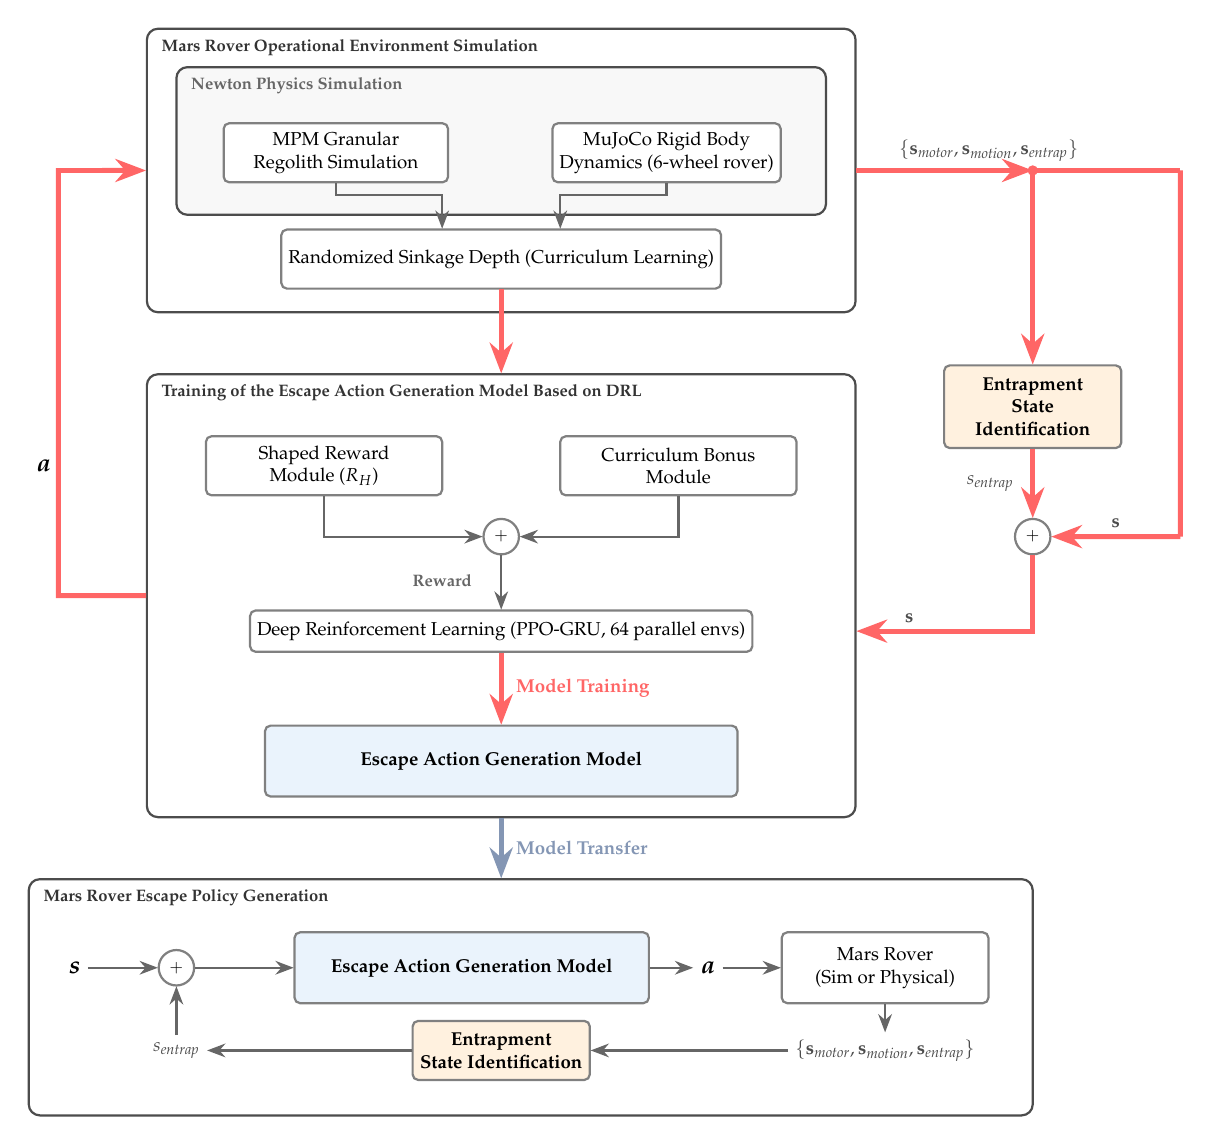
\begin{tikzpicture}[
    scale=0.75, transform shape, % Adjusted scale and layout for clarity and fit
    % Modern block styles ---
    outerbox/.style={rectangle, draw=black!70, thick, rounded corners=4pt,
                     inner sep=10pt},
    innerbox/.style={rectangle, draw=black!50, thick, fill=white,
                     minimum height=1cm, minimum width=3.8cm,
                     align=center, font=\small, rounded corners=2pt},
    orangebox/.style={innerbox, fill=lightorange!70,
                      font=\small\bfseries},
    bluebox/.style={innerbox, fill=lightblue!60,
                    font=\small\bfseries},
    redarrow/.style={-Stealth, line width=1.8pt, color=red!60},
    bluearrow/.style={-Stealth, line width=1.8pt, color=headerblue!60},
    arrow/.style={-Stealth, thick, color=black!60},
    circnode/.style={draw=black!50, circle, thick, minimum size=0.6cm,
                     inner sep=0pt, font=\footnotesize},
    lbl/.style={font=\small\itshape, text=black!70},
    boldlbl/.style={font=\large\bfseries\itshape},
    every node/.style={font=\small}
]

% ═══════════ TOP: SIMULATION ENVIRONMENT ═══════════
\node[outerbox, fill=white, minimum width=12cm, minimum height=4.8cm] (simbox) at (0, 12.5) {};
\node[font=\footnotesize\bfseries, anchor=north west, text=black!80]
    at ([xshift=4pt, yshift=-2pt]simbox.north west)
    {Mars Rover Operational Environment Simulation};

\node[outerbox, fill=boxgray, minimum width=11cm, minimum height=2.5cm] (physbox) at (0, 13.0) {};
\node[font=\footnotesize\bfseries, anchor=north west, text=black!60]
    at ([xshift=4pt, yshift=-2pt]physbox.north west) {Newton Physics Simulation};

\node[innerbox] (mpm) at (-2.8, 12.8) {MPM Granular\\Regolith Simulation};
\node[innerbox] (rigid) at (2.8, 12.8) {MuJoCo Rigid Body\\Dynamics (6-wheel rover)};
\node[innerbox, minimum width=7cm] (terrain) at (0, 11.0) {Randomized Sinkage Depth (Curriculum Learning)};
% ═══════════ RIGHT: ENTRAPMENT DETECTOR ═══════════
\node[orangebox, minimum width=3cm, minimum height=1.4cm] (entrapid) at (9, 8.5) {\textbf{Entrapment}\\State\\Identification};

% ═══════════ MIDDLE: TRAINING BLOCK ═══════════
\node[outerbox, fill=white, minimum width=12cm, minimum height=7.5cm] (trainbox) at (0, 5.3) {};
\node[font=\footnotesize\bfseries, anchor=north west, text=black!80]
    at ([xshift=4pt, yshift=-2pt]trainbox.north west)
    {Training of the Escape Action Generation Model Based on DRL};

\node[innerbox, minimum width=4cm] (handrew) at (-3, 7.5) {Shaped Reward\\Module ($R_H$)};
\node[innerbox, minimum width=4cm] (curricrew) at (3, 7.5) {Curriculum Bonus\\Module};
\node[circnode] (plus) at (0, 6.3) {$+$};
% \node[below=0.2cm of plus, font=\footnotesize\bfseries, text=black!60] {Reward};
\node[below=0.2cm of plus, xshift=-1.0cm, font=\footnotesize\bfseries, text=black!60] {Reward};
\node[innerbox, minimum width=8cm, minimum height=0.7cm] (drl) at (0, 4.7) {Deep Reinforcement Learning (PPO-GRU, 64 parallel envs)};

% State Concat
\node[circnode] (sconcat) at (9, 6.3) {$+$};

% Action
\node[boldlbl, anchor=east] (abig) at (-7.5, 7.5) {$\boldsymbol{a}$};

% Model Output
\vspace{1cm}
\node[bluebox, minimum width=8cm, minimum height=1.2cm] (escapemodel) at (0, 2.5) {\textbf{Escape Action Generation Model}};

% Connections (Top Half)
\draw[arrow] (mpm.south) -- ++(0,-0.2) -| ([xshift=-1cm]terrain.north);
\draw[arrow] (rigid.south) -- ++(0,-0.2) -| ([xshift=1cm]terrain.north);
\draw[redarrow] (terrain.south) -- (trainbox.north); % just touches Block 2 top
% Blue horizontal arrow from Block 1: split at midpoint, extends to tip
\coordinate (split) at (9, 12.5);
\coordinate (hTip)  at (11.5, 12.5);
\draw[redarrow]
    (simbox.east) -- (split)
    node[pos=0.75, above, font=\small\itshape, text=black!70]
        {$\{\mathbf{s}_{\text{motor}}, \mathbf{s}_{\text{motion}}, \mathbf{s}_{\text{entrap}}\}$};
\draw[redarrow, -{} ] (split) -- (hTip);
\fill[red!60] (split) circle (2.5pt);

% Midpoint → Entrapment State ID (vertical drop) — red bold
\draw[redarrow] (split) -- (entrapid.north);

% S_entrap: single vertical arrow, label shifted left
\draw[redarrow] (entrapid.south) -- (sconcat.north)
    node[midway, left=5pt, font=\small\itshape, text=black!70] {$s_{\text{entrap}}$};

% Tip → down → left → sconcat right side (bypass carrying s)
\draw[redarrow, -{}] (hTip) -- (11.5, 6.3);
\draw[redarrow] (11.5, 6.3) -- (sconcat.east)
    node[midway, above, font=\small\itshape, text=black!70] {$\mathbf{s}$};

% sconcat → trainbox right edge: drop vertically then go left (L-shape)
\draw[redarrow] (sconcat.south) -- (sconcat.south |- drl) -- (trainbox.east |- drl)
    node[pos=0.7, above, font=\small\itshape, text=black!70] {$\mathbf{s}$};

\draw[arrow] (handrew.south) |- (plus.west);
\draw[arrow] (curricrew.south) |- (plus.east);
\draw[arrow] (plus.south) -- (drl.north);
\draw[redarrow] (trainbox.west) -- (-7.5, 5.3) -- (-7.5, 12.5) -- (simbox.west); % Block 2 → a → Block 1 (red)

\draw[redarrow] (drl.south) -- (escapemodel.north) node[midway, right=3pt, font=\small\bfseries, text=red!60] {Model Training};

% ═══════════ BOTTOM: DEPLOYMENT ═══════════
\node[outerbox, fill=white, minimum width=17cm, minimum height=4cm] (deploybox) at (0.5, -1.5) {};
\node[font=\footnotesize\bfseries, anchor=north west, text=black!80]
    at ([xshift=4pt, yshift=-2pt]deploybox.north west)
    {Mars Rover Escape Policy Generation};

\node[circnode] (sconcat2) at (-5.5, -1.0) {$+$};
\node[boldlbl, anchor=east] (slbl2) at (-7.0, -1.0) {$\boldsymbol{s}$};
\node[bluebox, minimum width=6cm, minimum height=1.2cm] (escapemodel2) at (-0.5, -1.0) {\textbf{Escape Action Generation Model}};
\node[boldlbl] (abig2) at (3.5, -1.0) {$\boldsymbol{a}$};
\node[innerbox, minimum width=3.5cm, minimum height=1.2cm] (physical) at (6.5, -1.0) {Mars Rover\\(Sim or Physical)};
\node[orangebox, minimum width=3cm, minimum height=1cm] (entrapid2) at (0, -2.4) {\textbf{Entrapment}\\State Identification};
\node[lbl] (sabn2) at (-5.5, -2.4) {$s_{\text{entrap}}$};
\node[lbl] (stateout2) at (6.5, -2.4) {$\{\mathbf{s}_{\text{motor}}, \mathbf{s}_{\text{motion}}, \mathbf{s}_{\text{entrap}}\}$};

% Model Transfer: Block 2 bottom → Block 3 top (just touching)
\draw[bluearrow] (trainbox.south) -- (trainbox.south |- deploybox.north) node[midway, right=3pt, font=\small\bfseries, text=headerblue!60] {Model Transfer};

% Deploy connections
\draw[arrow] (slbl2.east) -- (sconcat2.west);
\draw[arrow] (sabn2.north) -- (sconcat2.south);
\draw[arrow] (sconcat2.east) -- (escapemodel2.west);
\draw[arrow] (escapemodel2.east) -- (abig2.west);
\draw[arrow] (abig2.east) -- (physical.west);
\draw[arrow] (physical.south) -- (stateout2.north);
\draw[arrow] (stateout2.west) -- (entrapid2.east);
\draw[arrow] (entrapid2.west) -- (sabn2.east);

\end{tikzpicture}
\caption{Escape policy generation method. Top: the training pipeline in simulation with reward shaping and curriculum learning. Bottom: the deployment pipeline on the physical or simulated Mars rover.}
\label{fig:escape_policy_generation}
\end{figure}


% ═══════════════════════════════════════════════════════════════════
% FIG: SIMULATION FRAMEWORK — exact replica of Bi & Ding Fig.10
% adapted for 6-wheel Mars rover
% ═══════════════════════════════════════════════════════════════════

\newpage
Figure~\ref{fig:simulation_framework} shows the simulation framework for our 6-wheel Mars rover with MPM granular terrain.

\begin{figure}[H]
\centering
\resizebox{\linewidth}{!}{%
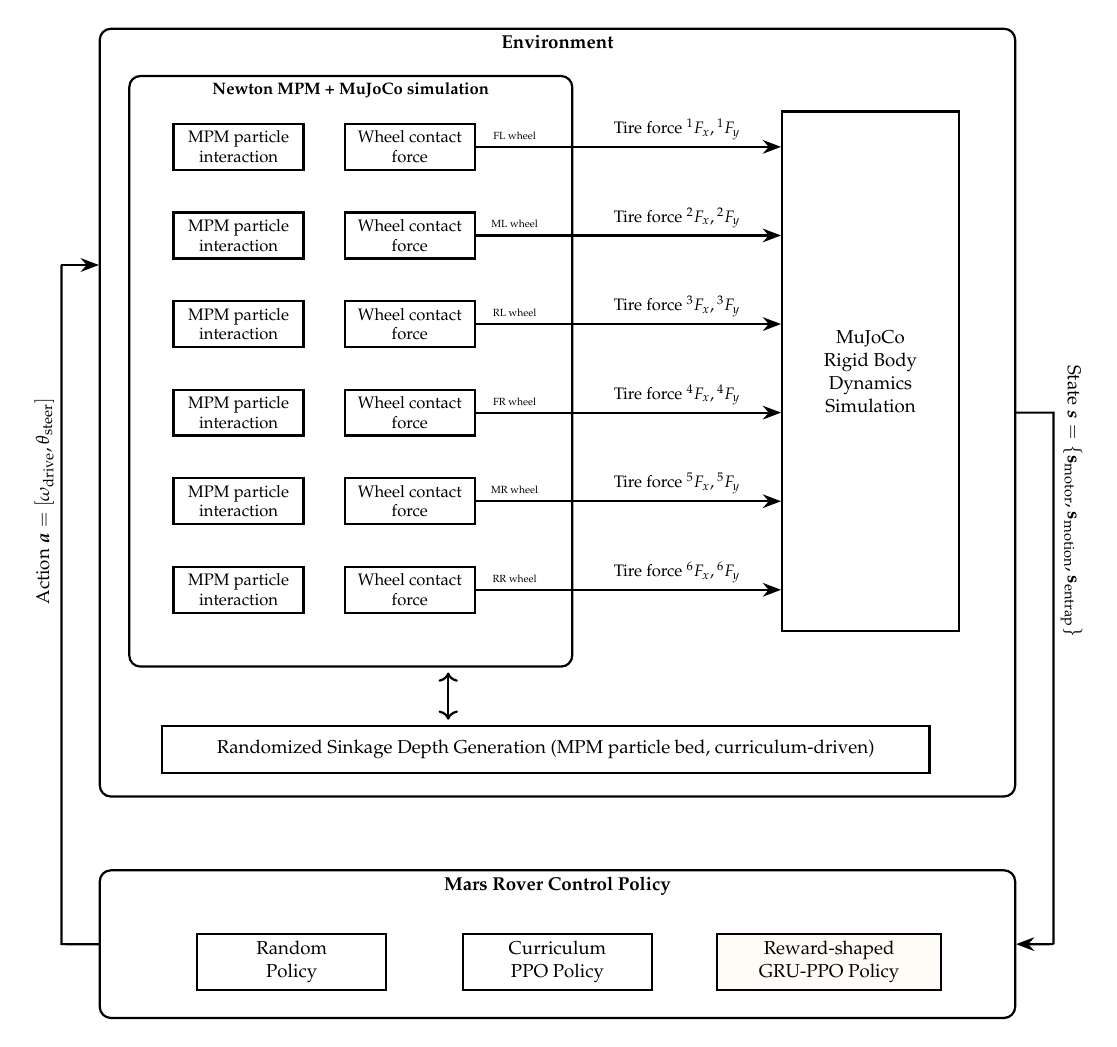
\begin{tikzpicture}[
    scale=0.75, transform shape,
    outerbox/.style={rectangle, draw=black, thick, rounded corners},
    innerbox/.style={rectangle, draw=black, thick, fill=lightblue!30, minimum height=0.8cm, align=center, font=\small},
    wheelbox/.style={rectangle, draw=black, thick, fill=white, minimum height=0.7cm, minimum width=2.2cm, align=center, font=\footnotesize},
    arrow/.style={-Stealth, thick},
    every node/.style={font=\small}
]

% --- Outer: Environment ---
\node[outerbox, fill=white, minimum width=15.5cm, minimum height=13cm,
      label={[font=\small\bfseries, anchor=north]north:Environment}]
      (envbox) at (0.2, 0.5) {};

% --- Inner: Simulation Box ---
\node[outerbox, fill=white, minimum width=7.5cm, minimum height=10cm,
      label={[font=\footnotesize\bfseries, anchor=north]north:Newton MPM + MuJoCo simulation}]
      (motorsim) at (-3.3, 1.2) {};

% --- SSMR rigid body dynamics box ---
\node[innerbox, minimum width=3cm, minimum height=8.8cm, fill=white] (rigidbody) at (5.5, 1.2) {MuJoCo\\Rigid Body\\Dynamics\\Simulation};

% 6 wheel rows
\foreach \i/\name/\ypos in {1/FL/5, 2/ML/3.5, 3/RL/2, 4/FR/0.5, 5/MR/-1, 6/RR/-2.5} {
    \node[wheelbox] (motor\i) at (-5.2, \ypos) {MPM particle\\interaction};
    \node[wheelbox] (tire\i) at (-2.3, \ypos) {Wheel contact\\force};

    % Calculate simulation box right boundary
    \coordinate (simright) at (motorsim.east |- tire\i.east);

    % --- Single Arrow from Wheel contact force to Rigid Body (one arrowhead at end) ---
    \draw[arrow] (tire\i.east) -- (rigidbody.west |- tire\i.east);

    % --- Wheel label inside simulation block (on top of arrow, before simright boundary) ---
    \node[font=\tiny, anchor=south] at ($(tire\i.east)!0.4!(simright)$) {\name{} wheel};

    % --- Tire Force label outside simulation block (on top of arrow, after simright boundary) ---
    \node[font=\footnotesize, anchor=south] at ($(simright)!0.5!(rigidbody.west |- tire\i.east)$) {Tire force ${}^{\i}F_x, {}^{\i}F_y$};
}

% Randomized terrain at bottom
\node[innerbox, minimum width=13cm, fill=white] (randterrain) at (0, -5.2) {Randomized Sinkage Depth Generation (MPM particle bed, curriculum-driven)};

% --- Vertical Bidirectional Arrow (VERTICAL - up/down) ---
\coordinate (arrowpos) at ($(motorsim.south)!0.5!(randterrain.north)$);
\draw[thick, <->] ($(arrowpos)+(0,-0.4)$) -- ($(arrowpos)+(0,0.4)$);

% ─── Bottom: Control policy (label centered at top) ───
\node[outerbox, fill=white, minimum width=15.5cm, minimum height=2.5cm,
      label={[font=\small\bfseries, anchor=north]north:Mars Rover Control Policy}]
      (policybox) at (0.2, -8.5) {};

\node[innerbox, fill=white, minimum width=3.2cm] (expert) at (-4.3, -8.8) {Random\\Policy};
\node[innerbox, fill=white, minimum width=3.2cm] (imitator) at (0.2, -8.8) {Curriculum\\PPO Policy};
\node[innerbox, fill=lightorange!20, minimum width=3.8cm] (fusion) at (4.8, -8.8) {Reward-shaped\\GRU-PPO Policy};

% ─── Action Feedback Loop (to Environment outer box) ───
\draw[thick] (policybox.west) -- (-8.2, -8.5) -- (-8.2, 3);
\draw[arrow] (-8.2, 3) -- (envbox.west |- -8.2, 3);
\node[font=\small, rotate=90, anchor=south] at (-8.2, -1) {Action $\boldsymbol{a} = [\omega_{\text{drive}}, \theta_{\text{steer}}]$};

% ─── State Feedback Loop (from Environment outer box) ───
\draw[thick] (envbox.east) -- (8.6, 0.5) -- (8.6, -8.5);
\draw[arrow] (8.6, -8.5) -- (policybox.east);
\node[font=\small, rotate=-90, anchor=south] at (8.6, -1) {State $\boldsymbol{s} = \{\mathbf{s}_{\text{motor}}, \mathbf{s}_{\text{motion}}, \mathbf{s}_{\text{entrap}}\}$};

\end{tikzpicture}
}% end resizebox
\caption{Simulation framework. The framework couples 6-wheel MPM particle interactions with granular sinkage via Newton MPM, and incorporates curriculum-driven sinkage depth randomization.}
\label{fig:simulation_framework}
\end{figure}

\newpage
% ═══════════════════════════════════════════════════════════════════
% FIG: POLICY NETWORK — exact replica of Bi & Ding Fig.8
% adapted for GRU instead of LSTM, 29D input, 10D output
% ═══════════════════════════════════════════════════════════════════

\newpage
Figure~\ref{fig:policy_network} shows the control policy network structure. We use GRU for reduced complexity, with 29D input and 10D actions (6 drive + 4 steer).

\begin{figure}[H]
\centering
\resizebox{\linewidth}{!}{%
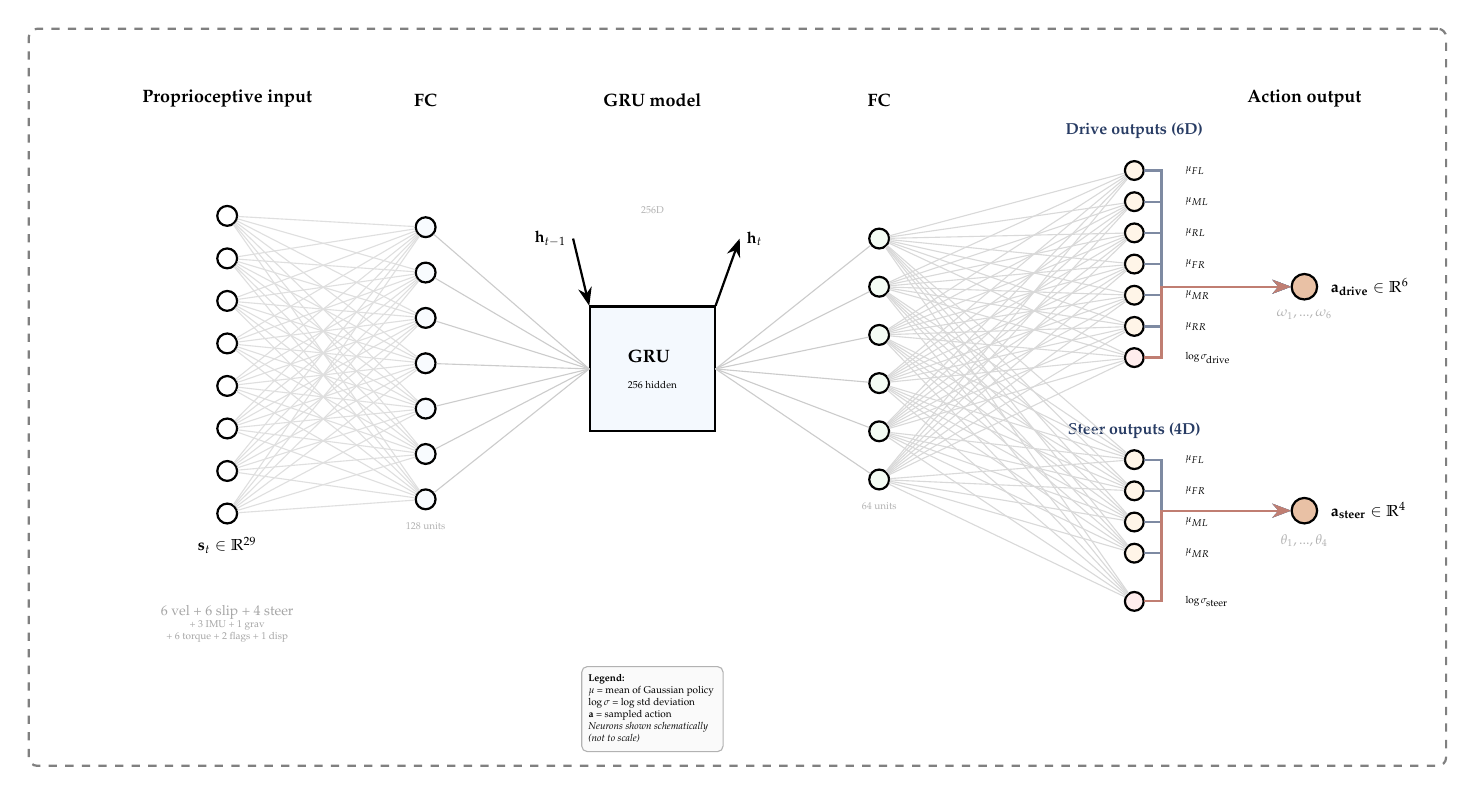
\begin{tikzpicture}[
    scale=0.72, transform shape,
    neuron/.style={circle, draw=black, thick, minimum size=0.35cm, fill=white},
    grubox/.style={rectangle, draw=black, thick, fill=lightblue!30, minimum width=1.8cm, minimum height=1.2cm, align=left, font=\small},
    arrow/.style={-Stealth, thick},
    dashedbox/.style={rectangle, draw=black!50, dashed, thick, rounded corners=3pt},
    every node/.style={font=\small}
]

% ─── Dashed outer box ───
\node[dashedbox, minimum width=25cm, minimum height=13cm, fill=white] at (9.5, 0) {};

% ─── Column labels ───
\node[font=\small\bfseries, anchor=south] at (0.5, 5) {Proprioceptive input};
\node[font=\small\bfseries, anchor=south] at (4, 5) {FC};
\node[font=\small\bfseries, anchor=south] at (8, 5) {GRU model};
\node[font=\small\bfseries, anchor=south] at (12, 5) {FC};
\node[font=\small\bfseries, anchor=south] at (19.5, 5) {Action output};

% ─── Input layer (29D) ───
\foreach \i in {1,...,8} {
    \pgfmathsetmacro{\ypos}{3.2 - (\i-1)*0.75}
    \node[neuron] (in\i) at (0.5, \ypos) {};
}
\node[font=\footnotesize, below=0.1cm of in8] {$\mathbf{s}_t \in \mathbb{R}^{29}$};
\node[font=\tiny, text=gray!70, align=center] at (0.5, -4.0) {\scriptsize 6 vel + 6 slip + 4 steer\\ + 3 IMU + 1 grav\\ + 6 torque + 2 flags + 1 disp};

% ─── FC1 layer (128 units) ───
\foreach \i in {1,...,7} {
    \pgfmathsetmacro{\ypos}{3 - (\i-1)*0.8}
    \node[neuron, fill=lightblue!20] (fc1\i) at (4, \ypos) {};
}
\node[font=\tiny, text=gray!60, below=0.1cm of fc17] {128 units};

% Connections input → FC1 (sparse for clarity)
\foreach \i in {1,...,8} {
    \foreach \j in {1,...,7} {
        \draw[gray!25] (in\i) -- (fc1\j);
    }
}

% ─── GRU block ───
\node[grubox, minimum width=2.2cm, minimum height=2.2cm, fill=lightblue!30] (gru) at (8, 0.5) {\textbf{GRU}\\[2pt]\tiny 256 hidden};

% Hidden state arrows with dimension labels
\node[font=\footnotesize\itshape] (ht_in) at (6.2, 2.8) {$\mathbf{h}_{t-1}$};
\draw[arrow] (ht_in.east) -- (gru.north west);
\node[font=\footnotesize\itshape] (ht_out) at (9.8, 2.8) {$\mathbf{h}_{t}$};
\draw[arrow] (gru.north east) -- (ht_out.west);
\node[font=\tiny, text=gray!60] at (8, 3.3) {256D};

% FC1 → GRU
\foreach \i in {1,...,7} {
    \draw[gray!40] (fc1\i) -- (gru.west);
}

% ─── FC2 layer (64 units) ───
\foreach \i in {1,...,6} {
    \pgfmathsetmacro{\ypos}{2.8 - (\i-1)*0.85}
    \node[neuron, fill=lightgreen!30] (fc2\i) at (12, \ypos) {};
}
\node[font=\tiny, text=gray!60, below=0.1cm of fc26] {64 units};

% GRU → FC2
\foreach \i in {1,...,6} {
    \draw[gray!40] (gru.east) -- (fc2\i);
}

% ─── Output: Drive branch (6 wheels) ───
% Mean outputs for 6 drive wheels
\node[font=\footnotesize\bfseries, text=deepblue] at (16.5, 4.7) {Drive outputs (6D)};
\foreach \i/\name in {1/FL, 2/ML, 3/RL, 5/MR, 6/RR} {
    \pgfmathsetmacro{\ypos}{4.0 - (\i-1)*0.55}
    \node[neuron, fill=lightorange!50, minimum size=0.3cm] (mu_drive\i) at (16.5, \ypos) {};
    \node[font=\tiny, right=0.6cm of mu_drive\i] {$\mu_{\name}$};
}
% µFR at original position (4.0 - 3*0.55 = 2.35)
\node[neuron, fill=lightorange!50, minimum size=0.3cm] (mu_drive4) at (16.5, 2.35) {};
\node[font=\tiny, right=0.6cm of mu_drive4] {$\mu_{FR}$};

% Log std for drive
\node[neuron, fill=lightred!50, minimum size=0.3cm] (logstd_drive) at (16.5, 0.7) {};
\node[font=\tiny, right=0.6cm of logstd_drive] {$\log\sigma_{\text{drive}}$};

% Drive action sampling
\node[neuron, fill=accentorange!40, minimum size=0.45cm] (a_drive) at (19.5, 1.95) {};
\node[font=\footnotesize\bfseries, right=0.1cm of a_drive] {$\mathbf{a}_{\text{drive}} \in \mathbb{R}^6$};
\node[font=\tiny, text=gray!60, below=0.05cm of a_drive] {\scriptsize $\omega_1,...,\omega_6$};

% ─── Output: Steer branch (4 wheels) ───
% Mean outputs for 4 steer joints
\node[font=\footnotesize\bfseries, text=deepblue] at (16.5, -0.6) {Steer outputs (4D)};
\foreach \i/\name in {1/FL, 2/FR, 3/ML, 4/MR} {
    \pgfmathsetmacro{\ypos}{-1.1 - (\i-1)*0.55}
    \node[neuron, fill=lightorange!50, minimum size=0.3cm] (mu_steer\i) at (16.5, \ypos) {};
    \node[font=\tiny, right=0.6cm of mu_steer\i] {$\mu_{\name}$};
}

% Log std for steer
\node[neuron, fill=lightred!50, minimum size=0.3cm] (logstd_steer) at (16.5, -3.6) {};
\node[font=\tiny, right=0.6cm of logstd_steer] {$\log\sigma_{\text{steer}}$};

% Steer action sampling
\node[neuron, fill=accentorange!40, minimum size=0.45cm] (a_steer) at (19.5, -2.0) {};
\node[font=\footnotesize\bfseries, right=0.1cm of a_steer] {$\mathbf{a}_{\text{steer}} \in \mathbb{R}^4$};
\node[font=\tiny, text=gray!60, below=0.05cm of a_steer] {\scriptsize $\theta_1,...,\theta_4$};

% ─── Connections FC2 to outputs (fully connected) ───
% To all drive means
\foreach \i in {1,...,6} {
    \foreach \j in {1,...,6} {
        \draw[gray!30] (fc2\i) -- (mu_drive\j);
    }
}
% To all steer means
\foreach \i in {1,...,6} {
    \foreach \j in {1,...,4} {
        \draw[gray!30] (fc2\i) -- (mu_steer\j);
    }
}
% To log stds
\foreach \i in {1,...,6} {
    \draw[gray!30] (fc2\i) -- (logstd_drive);
    \draw[gray!30] (fc2\i) -- (logstd_steer);
}

% ─── Gaussian sampling arrows ───
% Drive branch — all 6 means + logstd → a_drive
\foreach \i in {1,...,6} {
    \draw[arrow, color=deepblue!60] (mu_drive\i.east) -- ++(0.3,0) |- (a_drive.west);
}
\draw[arrow, color=marsred!60] (logstd_drive.east) -- ++(0.3,0) |- (a_drive.west);

% Steer branch — all 4 means + logstd → a_steer
\foreach \i in {1,...,4} {
    \draw[arrow, color=deepblue!60] (mu_steer\i.east) -- ++(0.3,0) |- (a_steer.west);
}
\draw[arrow, color=marsred!60] (logstd_steer.east) -- ++(0.3,0) |- (a_steer.west);

% ─── Legend box ───
\node[draw=gray!60, fill=lightgray!30, rounded corners=2pt, align=left, font=\tiny] at (8, -5.5) {
    \begin{tabular}{@{}l@{}}
    \textbf{Legend:}\\
    $\mu$ = mean of Gaussian policy\\
    $\log\sigma$ = log std deviation\\
    $\mathbf{a}$ = sampled action\\
    \textit{Neurons shown schematically}\\
    \textit{(not to scale)}
    \end{tabular}
};

\end{tikzpicture}
}% end resizebox
\caption{Structure of the Mars rover control policy network. The GRU (256 hidden units) processes 29D proprioceptive features (wheel velocities, slip ratios, steering angles, IMU data, gravity projection, drive torques, entrapment flags, and displacement) and outputs 10D actions: 6 independent drive velocities ($\omega_{\text{FL}}, \omega_{\text{ML}}, \omega_{\text{RL}}, \omega_{\text{FR}}, \omega_{\text{MR}}, \omega_{\text{RR}}$) and 4 steering angles ($\theta_{\text{FL}}, \theta_{\text{FR}}, \theta_{\text{ML}}, \theta_{\text{MR}}$). Actions are sampled from Gaussian distributions parameterized by the network. \textit{Neurons shown schematically, not to scale.}}
\label{fig:policy_network}
\end{figure}

\newpage
% ═══════════════════════════════════════════════════════════════════
% FIG: DRL BLOCK DIAGRAM — exact replica of Bi & Ding Fig.9
% adapted for our PPO-GRU training loop
% ═══════════════════════════════════════════════════════════════════
\vspace{15cm}
Figure~\ref{fig:drl_block_diagram} shows the block diagram of the reward-shaped DRL training loop.

\begin{figure}[H]
\centering
\begin{tikzpicture}[
    scale=0.78, transform shape,
    % --- Box Styles ---
    basebox/.style={rectangle, draw=black, thick, align=center, font=\small, minimum height=1cm},
    scheduler/.style={basebox, fill=blue!10, minimum width=3.2cm},
    env/.style={basebox, fill=orange!5, minimum width=4.5cm, minimum height=2.2cm},
    reward/.style={basebox, fill=white, minimum width=3cm},
    ppo/.style={basebox, fill=white, minimum width=5.5cm, minimum height=4.2cm},
    replay/.style={basebox, fill=gray!10, minimum width=1.8cm, minimum height=2.6cm, rounded corners=3pt},
    seq/.style={basebox, fill=gray!10, minimum width=10cm, minimum height=0.9cm, rounded corners=3pt},
    inner/.style={rectangle, draw=gray!40, fill=gray!5, align=center, font=\footnotesize, minimum height=0.8cm},
    % --- Arrow Styles ---
    arrow/.style={-Stealth, thick},
    dashedblue/.style={-Stealth, thick, dashed, color=blue!60},
    every node/.style={font=\small}
]

% ═══════════════════════════════════════════════════════════
% 1. TOP ROW: Config, Scheduler & Environment (Aligned at y=5.5)
% ═══════════════════════════════════════════════════════════

% Curriculum Config & Scheduler (Horizontally aligned)
\node[basebox, fill=gray!5, minimum width=2.2cm] (cfg) at (-8.5, 5.5) {Curriculum\\config};
\node[scheduler] (sched) at (-4.5, 5.5) {Curriculum\\Scheduler};
\draw[arrow] (cfg.east) -- (sched.west); % Clean horizontal arrow

% Stochastic Environment
\node[env] (env) at (4, 5.5) {};
\node[font=\small\bfseries, anchor=south] at (env.north) {Stochastic Environment};
\node[inner sep=0pt] at (4, 5.5) {
    
\includegraphics[width=3cm]{/home/mhpromit7473/regolith_entrapment_research/documentation/figures/newton_simulation.png}
};

% Legend (Aligned top-right)
\node[anchor=south east, font=\small\bfseries] at (8.5, 6.8) {Legend:};
\draw[arrow] (7.8, 6.4) -- (8.4, 6.4) node[right] {DRL process};
\draw[dashedblue] (7.8, 5.9) -- (8.4, 5.9) node[right] {Curriculum update};

% ═══════════════════════════════════════════════════════════
% 2. MIDDLE ROW: Reward & PPO
% ═══════════════════════════════════════════════════════════

% Reward Function
\node[reward] (reward) at (-2, 3) {Reward function};

% Clipped PPO Box
\node[ppo] (ppo) at (4, 0.8) {};
\node[font=\small\bfseries, anchor=north] at (ppo.north) {Clipped PPO (GRU)};

% PPO Internal Components
\node[inner, minimum width=1.9cm] (act) at (2.8, 1.6) {Actor\\(GRU)};
\node[inner, minimum width=1.9cm] (crit) at (4.8, 1.6) {Critic\\(GRU)};
\node[inner, minimum width=3.6cm, minimum height=1cm] (loss) at (4, 0.3)
    {PPO clip loss + value loss\\+ entropy loss};
\node[font=\tiny, text=gray!70, anchor=north] at ($(loss.south)+(0,-0.15)$) {Updating parameters with Adam/SGD};

% ═══════════════════════════════════════════════════════════
% 3. BOTTOM ROW: Replay & Sequence
% ═══════════════════════════════════════════════════════════

% Experience Replay Pool
\node[replay] (replay) at (-7, -0.5) {\rotatebox{90}{Experience replay pool}};

% Experience Sequence
\node[seq] (seq) at (-0.5, -3.5) {
    Experience sequence (max length $T$, GRU subsequence $= 16$)
};
\node[font=\scriptsize\itshape, text=gray!70] at (-0.5, -4.1) {
    $[(s_{t-T}, \dots, s_{t+1}), \dots, (s_t, a_t, r_t, s_{t+1})]$
};

% ═══════════════════════════════════════════════════════════
% 4. ARROW CONNECTIONS
% ═══════════════════════════════════════════════════════════

% A. Curriculum Updates (Blue Dashed)
\draw[dashedblue] (sched.east) -- (env.west |- sched.east)
    node[midway, above, text=blue!60] {Update $d_{\text{sinkage}}$};
\draw[dashedblue] (sched.south) -- (sched.south |- reward.west) -- (reward.west)
    node[pos=0.3, below, xshift=-1.2cm, text=blue!60] {Update weights};

% B. Environment → Reward
\draw[arrow] (env.west) -- ++(0,-0.8) -| (reward.north)
    node[pos=0.25, below, font=\footnotesize] {$(s_t, a_t)_\pi$};

% C. RL Closed Loop: Environment ↔ PPO
\draw[arrow] (env.south) -- (ppo.north)
    node[midway, left, font=\footnotesize] {$\mathbf{s}_t$};
\draw[arrow] (ppo.east) -- ++(1.0,0) coordinate(atmp) -- (atmp |- env.east) -- (env.east)
    node[pos=0.55, above, font=\footnotesize] {$\mathbf{a}_t$};

% D. Reward → PPO
\draw[arrow] (reward.south) |- (ppo.west)
    node[pos=0.25, left, font=\footnotesize] {$r_t$};

% E. PPO → Experience Sequence
\draw[arrow] (ppo.south) -- ++(0, -1.2) -| (seq.north)
    node[pos=0.0, right, font=\footnotesize] {$(s_t, a_t, r_t, s_{t+1})$};

% F. Experience Sequence → Replay Pool 
% FIXED: Routes to the left side (west), wrapping under the block to look like it comes from behind
\draw[arrow] (seq.west) -- ++(-3.5, 0) |- (replay.west);

% G. Replay Pool → PPO (Minibatch)
\draw[arrow] (replay.east) -- (ppo.west |- replay.east)
    node[midway, above, font=\footnotesize] {Minibatch};

\end{tikzpicture}
\caption{Block diagram of the reward-shaped DRL training loop. The curriculum scheduler updates environment difficulty and reward weights. The closed-loop interaction between PPO and the environment generates transitions, which are stored and sampled as minibatches for policy updates.}
\label{fig:drl_block_diagram}
\end{figure}

\newpage
% ─────── 3.1 Work Already Done ────────────────────────────────────
\subsection{Work Already Done}

\subsubsection{Simulation Environment}

The simulation environment couples two physics solvers through Newton's two-way coupling interface~\cite{newton}, as illustrated in Figure~\ref{fig:physics_stack}. The rigid-body solver follows the MuJoCo~\cite{todorov2012mujoco} CPU backend, while the granular solver uses SolverImplicitMPM based on the MPM formulation of Sulsky et al.~\cite{sulsky1994particle} with Drucker-Prager elastoplasticity for sand~\cite{klar2016sand}.

\begin{figure}[H]
\centering
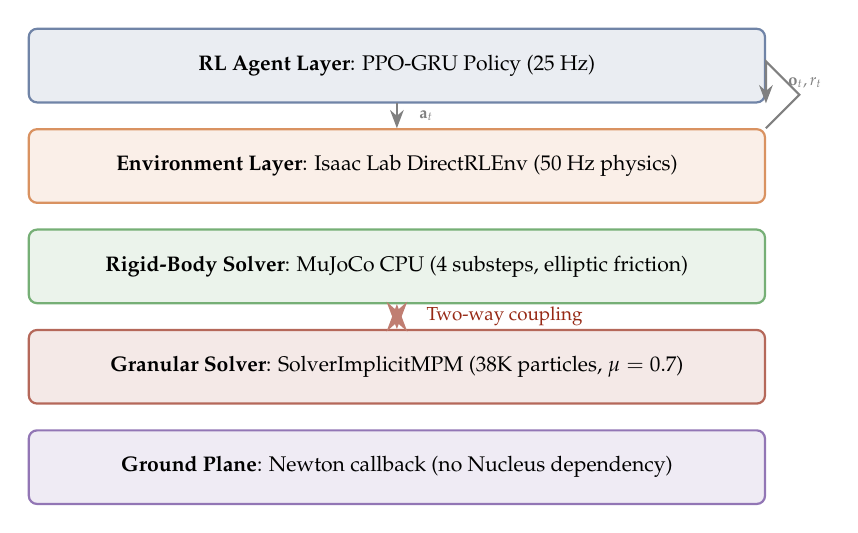
\begin{tikzpicture}[
    node distance=0.5cm,
    layer/.style={rectangle, draw=#1!70, fill=#1!10, thick, rounded corners=3pt,
                  minimum height=1.1cm, minimum width=11cm, align=center, font=\small},
    arrow/.style={-Stealth, thick, color=black!50},
    biarrow/.style={Stealth-Stealth, thick, color=marsred!60},
    scale=0.85, transform shape
]
\node[layer=headerblue] (rl) at (0,6) {\textbf{RL Agent Layer}: PPO-GRU Policy (25 Hz)};
\node[layer=accentorange] (env) at (0,4.5) {\textbf{Environment Layer}: Isaac Lab DirectRLEnv (50 Hz physics)};
\node[layer=softgreen] (rigid) at (0,3) {\textbf{Rigid-Body Solver}: MuJoCo CPU (4 substeps, elliptic friction)};
\node[layer=marsred] (mpm) at (0,1.5) {\textbf{Granular Solver}: SolverImplicitMPM (38K particles, $\mu=0.7$)};
\node[layer=softpurple] (ground) at (0,0) {\textbf{Ground Plane}: Newton callback (no Nucleus dependency)};
\draw[biarrow, line width=1.5pt] (rigid.south) -- (mpm.north)
    node[midway, right=0.3cm, font=\footnotesize, text=marsred] {Two-way coupling};
\draw[arrow] (rl.south) -- (env.north) node[midway, right=0.2cm, font=\scriptsize] {$\mathbf{a}_t$};
\draw[arrow] (env.north east) -- ++(0.5,0.5) -- ++(-0.5,0.5) -- (rl.south east)
    node[midway, right=0.2cm, font=\scriptsize] {$\mathbf{o}_t, r_t$};
\end{tikzpicture}
\caption{Physics simulation stack. The key innovation is two-way coupling between rigid-body dynamics and granular MPM particles.}
\label{fig:physics_stack}
\end{figure}

% ──── Placeholder for Newton sim screenshots ────
\begin{figure}[H]
\centering
\begin{subfigure}[b]{0.48\textwidth}
    \centering
    \imagePlaceholder[\linewidth]{5cm}{%
        \textbf{[Newton ViewerGL Screenshot]}\\[0.5em]
        Mars rover on MPM regolith bed\\
        (side view, particles visible)\\[0.3em]
        \texttt{eval.py --num\_envs 1}
    }
    \caption{Side view of rover on regolith}
\end{subfigure}
\hfill
\begin{subfigure}[b]{0.48\textwidth}
    \centering
    \imagePlaceholder[\linewidth]{5cm}{%
        \textbf{[Newton ViewerGL Screenshot]}\\[0.5em]
        Mars rover sinking into sand bed\\
        (isometric view, sinkage visible)\\[0.3em]
        \texttt{eval.py --num\_envs 1}
    }
    \caption{Isometric view showing wheel sinkage}
\end{subfigure}
\caption{Newton simulation environment showing the AAU 6-wheel Mars rover on granular regolith. The MPM particle bed (2.0\,m $\times$ 2.0\,m $\times$ 0.15\,m) provides realistic sinkage and wheel--sand interaction under Martian gravity (3.72\,m/s$^2$). Screenshots to be captured from Newton ViewerGL.}
\label{fig:newton_sim_screenshots}
\end{figure}

\newpage
Table~\ref{tab:env_params} summarizes the environment configuration.

\begin{tcolorbox}[dashedbox, left=0pt, right=0pt, top=4pt, bottom=4pt]
\begin{table}[H]
\centering
\caption{Environment configuration parameters}
\label{tab:env_params}
\small
\setlength{\tabcolsep}{6pt}
\renewcommand{\arraystretch}{1.4}
\begin{tabularx}{\textwidth}{>{\raggedright}p{3.8cm} >{\raggedright}p{4.2cm} X}
\toprule
\rowcolor{lightblue}
\textbf{Parameter} & \textbf{Value} & \textbf{Description} \\
\midrule
\multicolumn{3}{l}{\textbf{Simulation}} \\
Physics timestep & 0.02\,s (50\,Hz) & Simulation frequency \\
Policy decimation & 2 & Policy runs at 25\,Hz \\
Episode length & 20.0\,s (500 steps) & Maximum episode duration \\
Gravity & $(0,\,0,\,-3.72)$\,m/s$^2$ & Mars surface gravity \\
Parallel environments & 64 & Training environments \\
\midrule
\multicolumn{3}{l}{\textbf{Granular Material (MPM)}} \\
Voxel size & 0.05\,m & MPM grid resolution \\
Sand bed dimensions & 2.0\,m $\times$ 2.0\,m $\times$ 0.15\,m & Per-environment regolith bed \\
Particle count & $\sim$38{,}400 per env & Total granular particles \\
Friction coefficient $\mu$ & 0.7 & Wheel--sand friction \\
\midrule
\multicolumn{3}{l}{\textbf{Rigid-Body Solver}} \\
Solver & MuJoCo CPU & Rigid-body dynamics \\
Constraint iterations & 4 & Solver iterations per step \\
Substeps & 4 & Physics substeps per step \\
\midrule
\multicolumn{3}{l}{\textbf{Domain Randomization}} \\
Motor gain & $\mathcal{U}(0.8,\,1.2)$ & Multiplicative gain noise \\
Observation noise & $\mathcal{N}(0,\,0.02)$ & Additive Gaussian noise \\
Sinkage range & 0.08--0.15\,m & Curriculum-driven \\
Spawn yaw & $\pm 15^\circ$ & Random heading offset \\
\bottomrule
\end{tabularx}
\end{table}
\end{tcolorbox}

\newpage
\subsubsection{Robot Platform}

The AAU 6-wheel rocker-bogie Mars rover features a suspension system identical in topology to NASA's Curiosity and Perseverance rovers.

% ──── Placeholder for rover images ────
\begin{figure}[H]
\centering
\begin{subfigure}[b]{0.48\textwidth}
    \centering
    \imagePlaceholder[\linewidth]{5cm}{%
        \textbf{[Rover USD Render]}\\[0.5em]
        AAU Mars Rover (Mars\_Rover.usd)\\
        6-wheel rocker-bogie suspension\\
        from RLRoverLab
    }
    \caption{Rover USD model}
\end{subfigure}
\hfill
\begin{subfigure}[b]{0.48\textwidth}
    \centering
    \imagePlaceholder[\linewidth]{5cm}{%
        \textbf{[Newton ViewerGL Screenshot]}\\[0.5em]
        Rover in simulation with\\
        MPM sand particles visible\\
        and wheel contact forces
    }
    \caption{Rover in Newton simulation}
\end{subfigure}
\caption{The AAU Mars rover platform used in simulation. (a) USD model render showing the 6-wheel rocker-bogie suspension. (b) Rover in Newton simulation environment with granular regolith particles.}
\label{fig:rover_platform}
\end{figure}

\begin{tcolorbox}[dashedbox, left=0pt, right=0pt, top=4pt, bottom=4pt]
\begin{table}[H]
\centering
\caption{AAU Mars rover joint configuration}
\label{tab:rover_joints}
\small
\setlength{\tabcolsep}{8pt}
\renewcommand{\arraystretch}{1.4}
\begin{tabularx}{\textwidth}{X >{\centering}p{1.6cm} >{\centering}p{2.4cm} >{\centering\arraybackslash}p{2.0cm}}
\toprule
\rowcolor{lightblue}
\textbf{Joint Type} & \textbf{Count} & \textbf{Control Mode} & \textbf{Range} \\
\midrule
Drive (continuous) & 6 & Velocity & $\pm 6$\,rad/s \\
Steer (revolute) & 4 & Position & $\pm 0.6$\,rad \\
Passive (rocker/diff.) & \textit{N} & Free (unactuated) & -- \\
\bottomrule
\multicolumn{4}{l}{\footnotesize Drive joints mapped to $[-1,1]$ $\to$ $\pm6$\,rad/s;\enspace steer joints mapped to $[-1,1]$ $\to$ $\pm0.6$\,rad.}
\end{tabularx}
\end{table}
\end{tcolorbox}

\newpage
\subsubsection{Observation and Action Spaces}

\begin{equation}
\mathbf{o}_t = \underbrace{[\mathbf{v}_{\text{wheel}}]}_{\text{6D}} \oplus \underbrace{[\boldsymbol{\sigma}_{\text{slip}}]}_{\text{6D}} \oplus \underbrace{[\boldsymbol{\theta}_{\text{steer}}]}_{\text{4D}} \oplus \underbrace{[\mathbf{a}_{\text{imu}}]}_{\text{3D}} \oplus \underbrace{[g_z]}_{\text{1D}} \oplus \underbrace{[\boldsymbol{\tau}_{\text{drive}}]}_{\text{6D}} \oplus \underbrace{[f_{\text{entrap}}]}_{\text{1D}} \oplus \underbrace{[f_{\text{anomaly}}]}_{\text{1D}} \oplus \underbrace{[d_{\text{norm}}]}_{\text{1D}}
\label{eq:obs_space}
\end{equation}

\begin{tcolorbox}[dashedbox, left=0pt, right=0pt, top=4pt, bottom=4pt]
\begin{table}[H]
\centering
\caption{Observation space components (29D total)}
\label{tab:obs_space}
\small
\setlength{\tabcolsep}{6pt}
\renewcommand{\arraystretch}{1.4}
\begin{tabularx}{\textwidth}{>{\raggedright}p{2.5cm} >{\centering}p{1.0cm} >{\centering}p{2.2cm} X}
\toprule
\rowcolor{lightblue}
\textbf{Component} & \textbf{Dim} & \textbf{Normalization} & \textbf{Description} \\
\midrule
\multicolumn{4}{l}{\textbf{Proprioception (Wheel)}} \\
$\mathbf{v}_{\text{wheel}}$ & 6 & $/\,6$\,rad/s & Drive joint angular velocities \\
$\boldsymbol{\sigma}_{\text{slip}}$ & 6 & $[0,\,1]$ & Per-wheel slip ratio \\
$\boldsymbol{\theta}_{\text{steer}}$ & 4 & $/\,0.6$\,rad & Steering joint positions \\
$\boldsymbol{\tau}_{\text{drive}}$ & 6 & $/\,\tau_{\max}$ & Normalized drive torques \\
\midrule
\multicolumn{4}{l}{\textbf{Inertial (IMU)}} \\
$\mathbf{a}_{\text{imu}}$ & 3 & $/\,g$ & Body linear acceleration \\
$g_z$ & 1 & $[-1,\,1]$ & Projected gravity z-component \\
\midrule
\multicolumn{4}{l}{\textbf{Detection Flags}} \\
$f_{\text{entrap}}$ & 1 & $\{0,\,1\}$ & Binary entrapment flag \\
$f_{\text{anomaly}}$ & 1 & $\{0,\,1\}$ & Binary torque anomaly flag \\
\midrule
\multicolumn{4}{l}{\textbf{Navigation}} \\
$d_{\text{norm}}$ & 1 & $/\,d_{\text{escape}}$ & Normalized $+X$ displacement \\
\midrule
\rowcolor{lightblue!40}\textbf{Total} & \textbf{29} & -- & -- \\
\bottomrule
\end{tabularx}
\end{table}
\end{tcolorbox}

The action space comprises 10 continuous dimensions:
\begin{equation}
\mathbf{a}_t = \underbrace{[\boldsymbol{\omega}_{\text{drive}}]}_{\text{6D: } [-1,1] \to \pm 6\,\text{rad/s}} \oplus \underbrace{[\boldsymbol{\theta}_{\text{steer}}]}_{\text{4D: } [-1,1] \to \pm 0.6\,\text{rad}}
\end{equation}


\subsubsection{Dual-Sensor Entrapment Detection}

Inspired by Bi and Ding~\cite{bi2026escape}, we implement two complementary detection mechanisms:

\textbf{Slip-based}: $f_{\text{entrap}} = \mathbb{I}\left[ |v_x| < 0.15\,\text{m/s} \wedge \bar{\sigma} > 0.5 \text{ for } 10\text{ steps} \right]$

\textbf{Torque-based}: $f_{\text{anomaly}} = \mathbb{I}\left[ \max_i |\tau_i/\tau_{\max}| > 0.8 \text{ for } 10\text{ steps} \right]$

\newpage
\subsubsection{Reward Function}

\begin{equation}
R_t = r_{\text{progress}} + r_{\text{escape}} + r_{\text{rocking}} - p_{\text{slip}} - p_{\text{tilt}} - p_{\text{smooth}} - p_{\text{abnormal}}
\end{equation}

\begin{tcolorbox}[dashedbox, left=0pt, right=0pt, top=4pt, bottom=4pt]
\begin{table}[H]
\centering
\caption{Reward function components (v3 methodology reference)}
\label{tab:reward}
\small
\setlength{\tabcolsep}{5pt}
\renewcommand{\arraystretch}{1.4}
\begin{tabularx}{\textwidth}{>{\raggedright}p{2.2cm} >{\centering}p{1.4cm} X >{\raggedright\arraybackslash}p{3.5cm}}
\toprule
\rowcolor{lightblue}
\textbf{Term} & \textbf{Weight} & \textbf{Formula} & \textbf{Purpose} \\
\midrule
\multicolumn{4}{l}{\textbf{Incentives}} \\
$r_{\text{progress}}$ & $+3.0$ & $v_x \cdot \Delta t$ & Forward motion reward \\
$r_{\text{escape}}$ & $+5.0$ & Milestones at $0.3$\,m & Shaped escape bonus \\
$r_{\text{rocking}}$ & $+2.0$ & $\Delta v_x \cdot f_{\text{entrap}} \cdot \Delta t$ & Velocity reversals when stuck \\
\midrule
\multicolumn{4}{l}{\textbf{Penalties}} \\
$p_{\text{slip}}$ & $-1.0$ & $\bar{\sigma}(1 - f_{\text{entrap}})\Delta t$ & Excessive wheel spin \\
$p_{\text{tilt}}$ & $-0.3$ & $\|\omega_{xy}\|_2 \cdot \Delta t$ & Body instability \\
$p_{\text{smooth}}$ & $-0.05$ & $\|\Delta \mathbf{a}\|_2 \cdot \Delta t$ & Jerky actions \\
$p_{\text{abnormal}}$ & $-0.5$ & $(-v_x)^+ \cdot f_{\text{anom}}(1{-}f_{\text{entrap}})\Delta t$ & Backward motion under anomaly \\
\bottomrule
\multicolumn{4}{l}{\footnotesize Note: v3 weights; v4 (Table~\ref{tab:reward_function}) uses updated values after tuning.}
\end{tabularx}
\end{table}
\end{tcolorbox}


\subsubsection{PPO Training Configuration}

\begin{tcolorbox}[dashedbox, left=0pt, right=0pt, top=4pt, bottom=4pt]
\begin{table}[H]
\centering
\caption{PPO training hyperparameters and GRU architecture}
\label{tab:ppo_config}
\small
\setlength{\tabcolsep}{6pt}
\renewcommand{\arraystretch}{1.4}
\begin{tabularx}{\textwidth}{X >{\centering}p{3.0cm} >{\raggedright\arraybackslash}p{5.0cm}}
\toprule
\rowcolor{lightblue}
\textbf{Parameter} & \textbf{Value} & \textbf{Notes} \\
\midrule
\multicolumn{3}{l}{\textbf{On-Policy Rollout}} \\
Rollout length & 32 steps & Data collected per update \\
Learning epochs & 5 & Passes over each rollout \\
Mini-batches & 4 & Gradient updates per epoch \\
\midrule
\multicolumn{3}{l}{\textbf{Optimization}} \\
Learning rate & $3 \times 10^{-4}$ & Adam optimizer \\
Clip ratio ($\varepsilon$) & 0.2 & PPO clipped surrogate \\
Discount ($\gamma$) & 0.99 & Future reward weighting \\
GAE lambda ($\lambda$) & 0.95 & Advantage estimation \\
Entropy coefficient & 0.03 & Prevents premature convergence \\
\midrule
\multicolumn{3}{l}{\textbf{GRU Architecture}} \\
GRU hidden size & 256 & Recurrent state dimension \\
GRU layers & 1 & Single recurrent layer \\
BPTT sequence length & 16 & Truncated backprop \\
\bottomrule
\end{tabularx}
\end{table}
\end{tcolorbox}


\subsubsection{Curriculum Learning}

\begin{equation}
d_{\text{sinkage}}(p) = d_{\min} + p \cdot (d_{\max} - d_{\min}), \quad p \in [0, 1]
\end{equation}
where $d_{\min} = 0.08$\,m and $d_{\max} = 0.15$\,m.


\subsubsection{Reward Tuning and Bug Fixes}
\label{sec:reward_tuning}

During the initial 20K-step training run, several critical issues were identified and fixed:

\paragraph{Slip penalty too high.} With weight 1.0, forward driving yielded \textit{negative} net reward:
\begin{align}
r_{\text{progress}} &= 3.0 \times 0.2 \times 0.02 = +0.012, \quad
p_{\text{slip}} = 1.0 \times 0.8 \times 0.02 = -0.016, \quad
\text{Net} = -0.004
\end{align}
Reduced to 0.3: Net $= +0.012 - 0.005 = +0.007$ (correct incentive).

\paragraph{Torque anomaly bug.} Original used \texttt{clamp(0,2)} killing negative torques and \texttt{mean()} diluting signal. Fixed with \texttt{abs()} and \texttt{max()} per wheel.

\paragraph{Backward-driving exploit.} Escape reward triggered for any direction. Fixed to require +X displacement with spawn yaw $\pm 15^\circ$.


% ─────── 3.2 Expected Work ────────────────────────────────────────
\subsection{Expected Work to Be Done}

\subsubsection{Phase 1: CNN-GRU Sinkage Detection Classifier}

\begin{figure}[H]
\centering
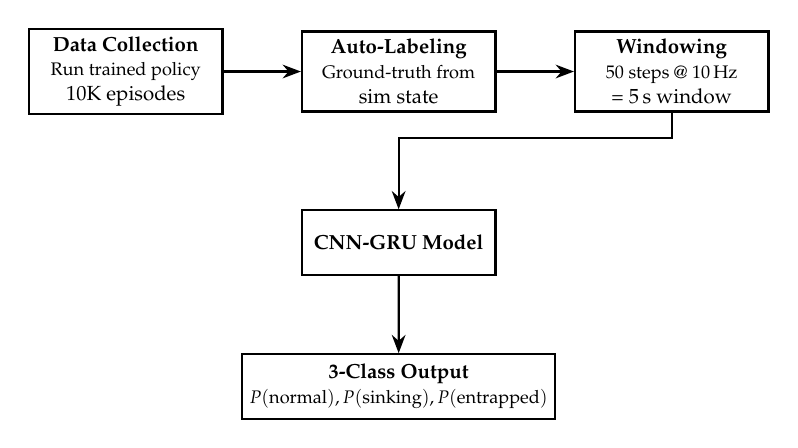
\begin{tikzpicture}[
    node distance=0.5cm and 1cm,
    box/.style={rectangle, draw=black, thick, fill=#1, minimum height=1cm, minimum width=3cm, align=center, font=\small},
    arrow/.style={-Stealth, thick},
    scale=0.82, transform shape
]
\node[box=white] (collect) at (0,0) {\textbf{Data Collection}\\\footnotesize Run trained policy\\10K episodes};
\node[box=white, right=1.2cm of collect] (label) {\textbf{Auto-Labeling}\\\footnotesize Ground-truth from\\sim state};
\node[box=white, right=1.2cm of label] (window) {\textbf{Windowing}\\\footnotesize 50 steps @ 10\,Hz\\= 5\,s window};
\node[box=white, below=1.5cm of label] (model) {\textbf{CNN-GRU Model}};
\node[box=white, below=1.2cm of model] (output) {\textbf{3-Class Output}\\\footnotesize $P(\text{normal}), P(\text{sinking}), P(\text{entrapped})$};
\draw[arrow] (collect) -- (label);
\draw[arrow] (label) -- (window);
\draw[arrow] (window.south) -- ++(0,-0.4) -| (model.north);
\draw[arrow] (model) -- (output);
\end{tikzpicture}
\caption{Planned CNN-GRU sinkage detection pipeline.}
\label{fig:detection_pipeline}
\end{figure}

Target: F1 $> 0.90$ on ``entrapped'' class, latency $< 1$\,s, inference $< 5$\,ms on RPi5.


\subsubsection{Scaling Training}

\begin{itemize}
    \item \textbf{RTX 4090} (24\,GB): 512 parallel environments, 2M timesteps
    \item Hyperparameter sweep: rollout length, entropy coefficient, learning rate (following~\cite{schulman2015gae})
    \item Multi-seed evaluation: 5 random seeds for statistical significance
    \item Ablation studies: GRU~\cite{cho2014gru} vs.\ MLP, dual detection vs.\ single, curriculum impact
    \item Comparison against SAC~\cite{haarnoja2018sac} and TRPO~\cite{schulman2015trpo} baselines
\end{itemize}


\subsubsection{Phase 3: Sim-to-Real Deployment}
\label{sec:sim2real}

\begin{figure}[H]
\centering
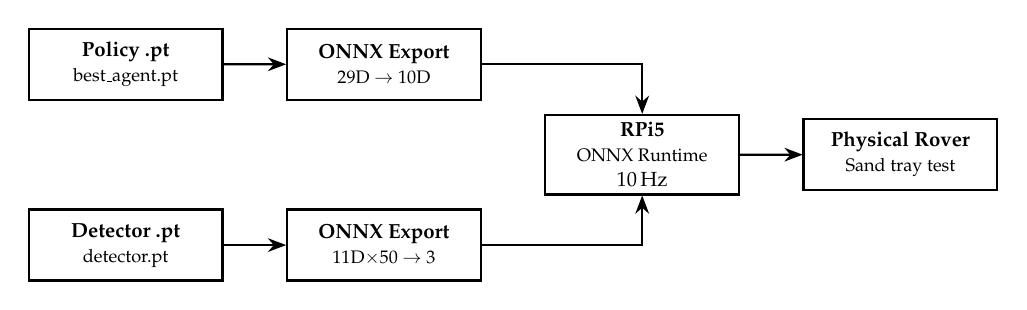
\begin{tikzpicture}[
    node distance=0.6cm and 1.2cm,
    box/.style={rectangle, draw=black, thick, fill=#1, minimum height=1.1cm, minimum width=3cm, align=center, font=\small},
    arrow/.style={-Stealth, thick},
    scale=0.82, transform shape
]
\node[box=white] (p1) at (0,2.8) {\textbf{Policy .pt}\\\footnotesize best\_agent.pt};
\node[box=white] (p2) at (0,0) {\textbf{Detector .pt}\\\footnotesize detector.pt};
\node[box=white] (o1) at (4,2.8) {\textbf{ONNX Export}\\\footnotesize 29D $\to$ 10D};
\node[box=white] (o2) at (4,0) {\textbf{ONNX Export}\\\footnotesize 11D$\times$50 $\to$ 3};
\node[box=white] (rpi) at (8,1.4) {\textbf{RPi5}\\\footnotesize ONNX Runtime\\10\,Hz};
\node[box=white] (hw) at (12,1.4) {\textbf{Physical Rover}\\\footnotesize Sand tray test};
\draw[arrow] (p1) -- (o1);
\draw[arrow] (p2) -- (o2);
\draw[arrow] (o1.east) -| (rpi.north);
\draw[arrow] (o2.east) -| (rpi.south);
\draw[arrow] (rpi) -- (hw);
\end{tikzpicture}
\caption{Planned sim-to-real deployment pipeline.}
\label{fig:deployment_pipeline}
\end{figure}


% ══════════════════════════════════════════════════════════════════
%                       4. RESULTS
% ══════════════════════════════════════════════════════════════════
\newpage
\section{Results}

Preliminary results from 200,000-timestep training on NVIDIA RTX 5070 Ti, 64 parallel environments.

\subsection{Training Overview}

\begin{figure}[H]
\centering
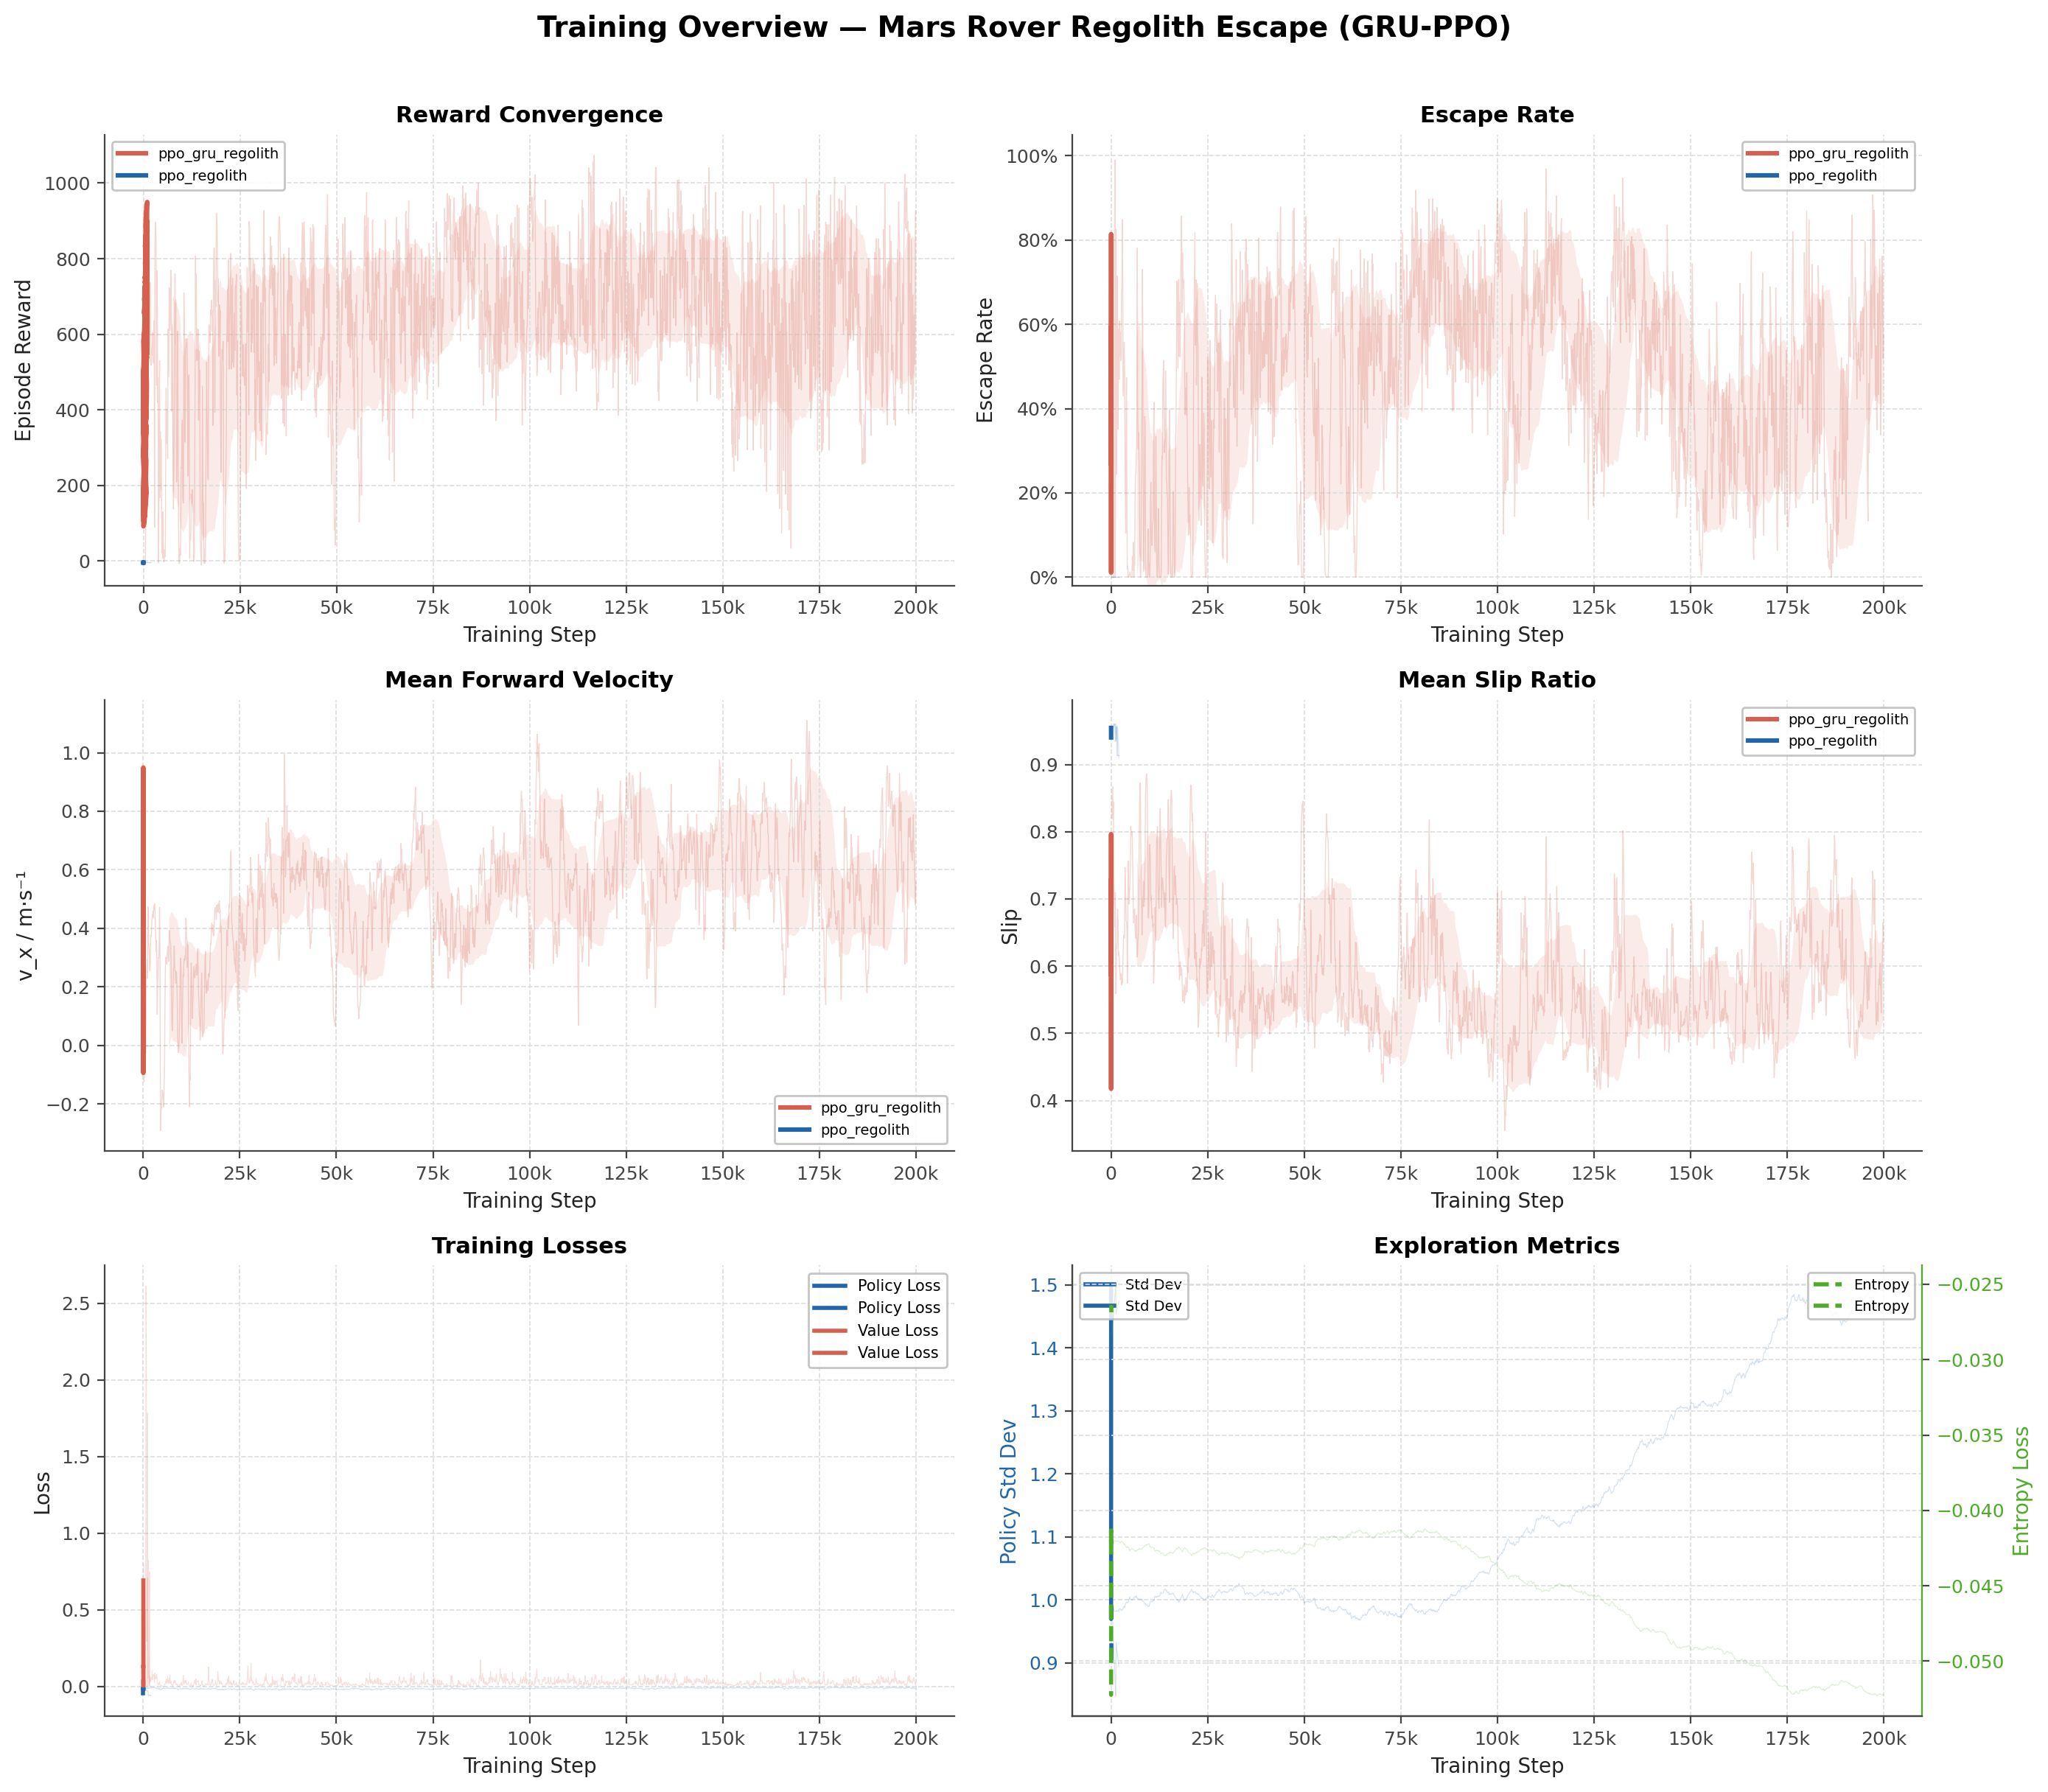
\includegraphics[width=0.98\textwidth]{figures/training_overview.png}
\caption{Training overview across 200K timesteps: reward convergence, escape rate, forward velocity, slip ratio, losses, and exploration metrics. GRU-PPO (red) vs.\ feedforward baseline (blue).}
\label{fig:training_overview}
\end{figure}

\subsection{Key Performance Metrics}

\begin{tcolorbox}[dashedbox, left=0pt, right=0pt, top=4pt, bottom=4pt]
\begin{table}[H]
\centering
\caption{Training results at 200{,}000 timesteps (RTX 5070 Ti, 64 parallel environments)}
\label{tab:results}
\small
\setlength{\tabcolsep}{6pt}
\renewcommand{\arraystretch}{1.4}
\begin{tabularx}{\textwidth}{X >{\centering}p{2.4cm} >{\centering}p{2.4cm} >{\centering\arraybackslash}p{2.8cm}}
\toprule
\rowcolor{lightblue}
\textbf{Metric} & \textbf{Value} & \textbf{Target} & \textbf{Status} \\
\midrule
Mean episode reward & $\sim$926 & $> 100$ & \textcolor{softgreen!60!black}{\textbf{$\checkmark$ Achieved}} \\
Mean forward velocity $v_x$ & 0.557\,m/s & $> 0.15$\,m/s & \textcolor{softgreen!60!black}{\textbf{$\checkmark$ Achieved}} \\
Curriculum progress & 1.0 & 1.0 & \textcolor{softgreen!60!black}{\textbf{$\checkmark$ Achieved}} \\
\midrule
Escape rate & $\sim$57\% & $> 70\%$ & \textcolor{marsred}{\textbf{$\nearrow$ In Progress}} \\
Policy std dev & 1.496 & $< 1.0$ & \textcolor{marsred}{\textbf{$\times$ Not Converged}} \\
\bottomrule
\multicolumn{4}{l}{\footnotesize Peak escape rate 99\% observed mid-training; requires 2M+ steps for stable convergence.}
\end{tabularx}
\end{table}
\end{tcolorbox}

\subsection{Reward Analysis}

\begin{figure}[H]
\centering
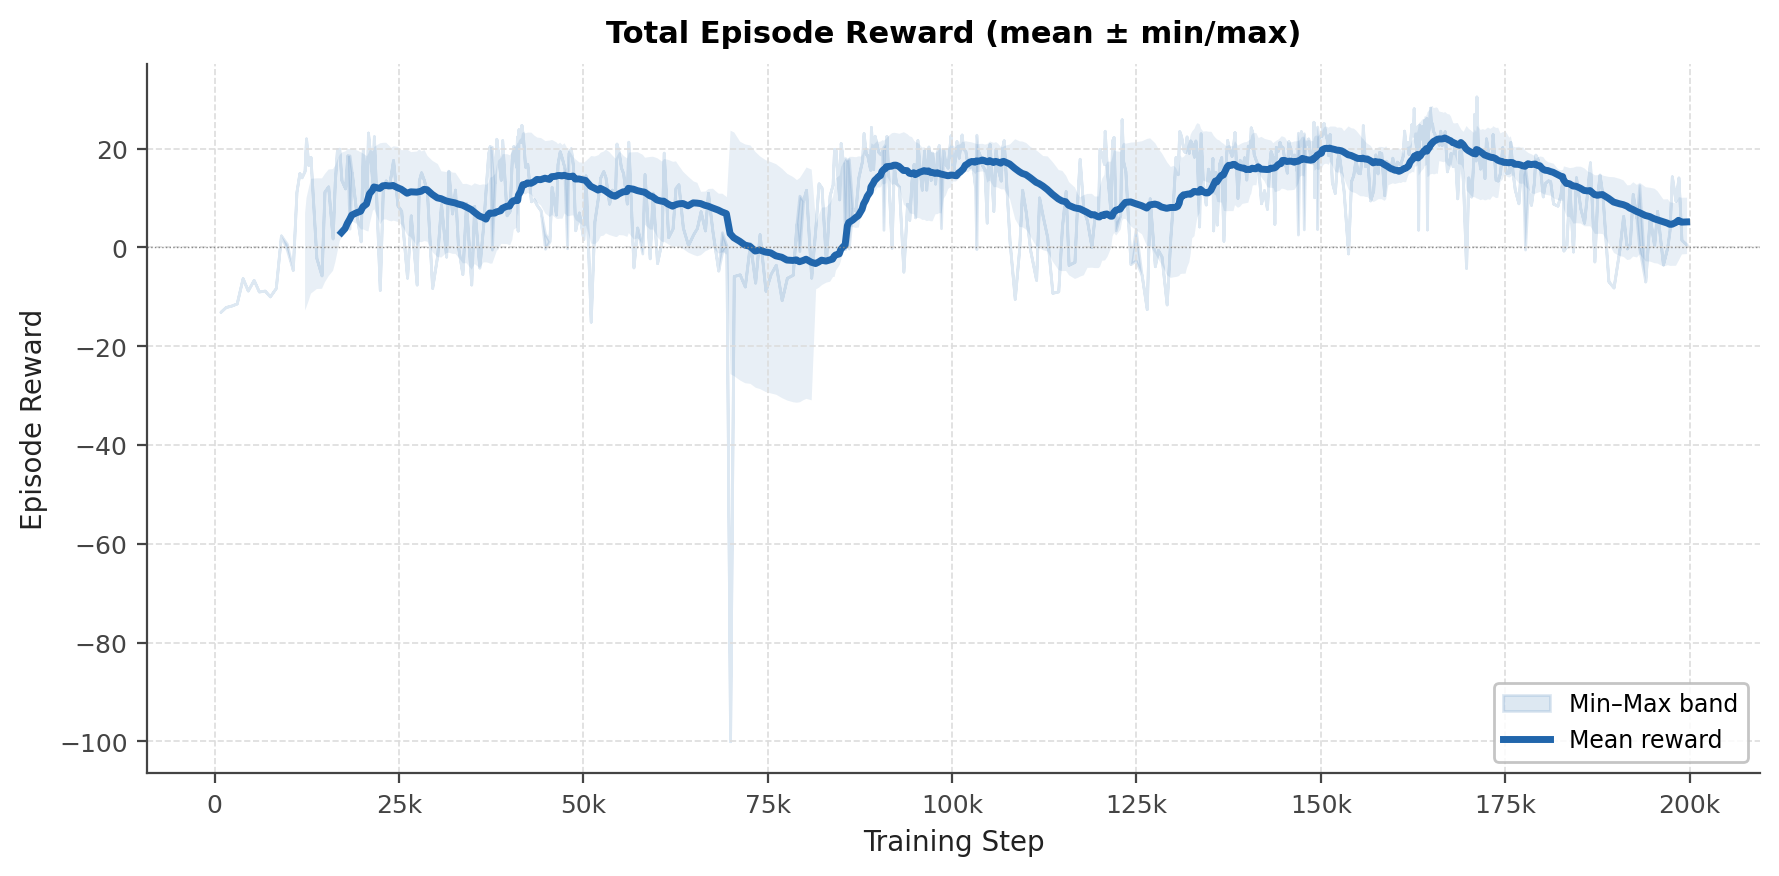
\includegraphics[width=0.95\textwidth]{figures/reward_breakdown.png}
\caption{Reward breakdown showing min, mean, and max episode rewards over training.}
\label{fig:reward_breakdown}
\end{figure}

\subsection{Environment Metrics}

\begin{figure}[H]
\centering
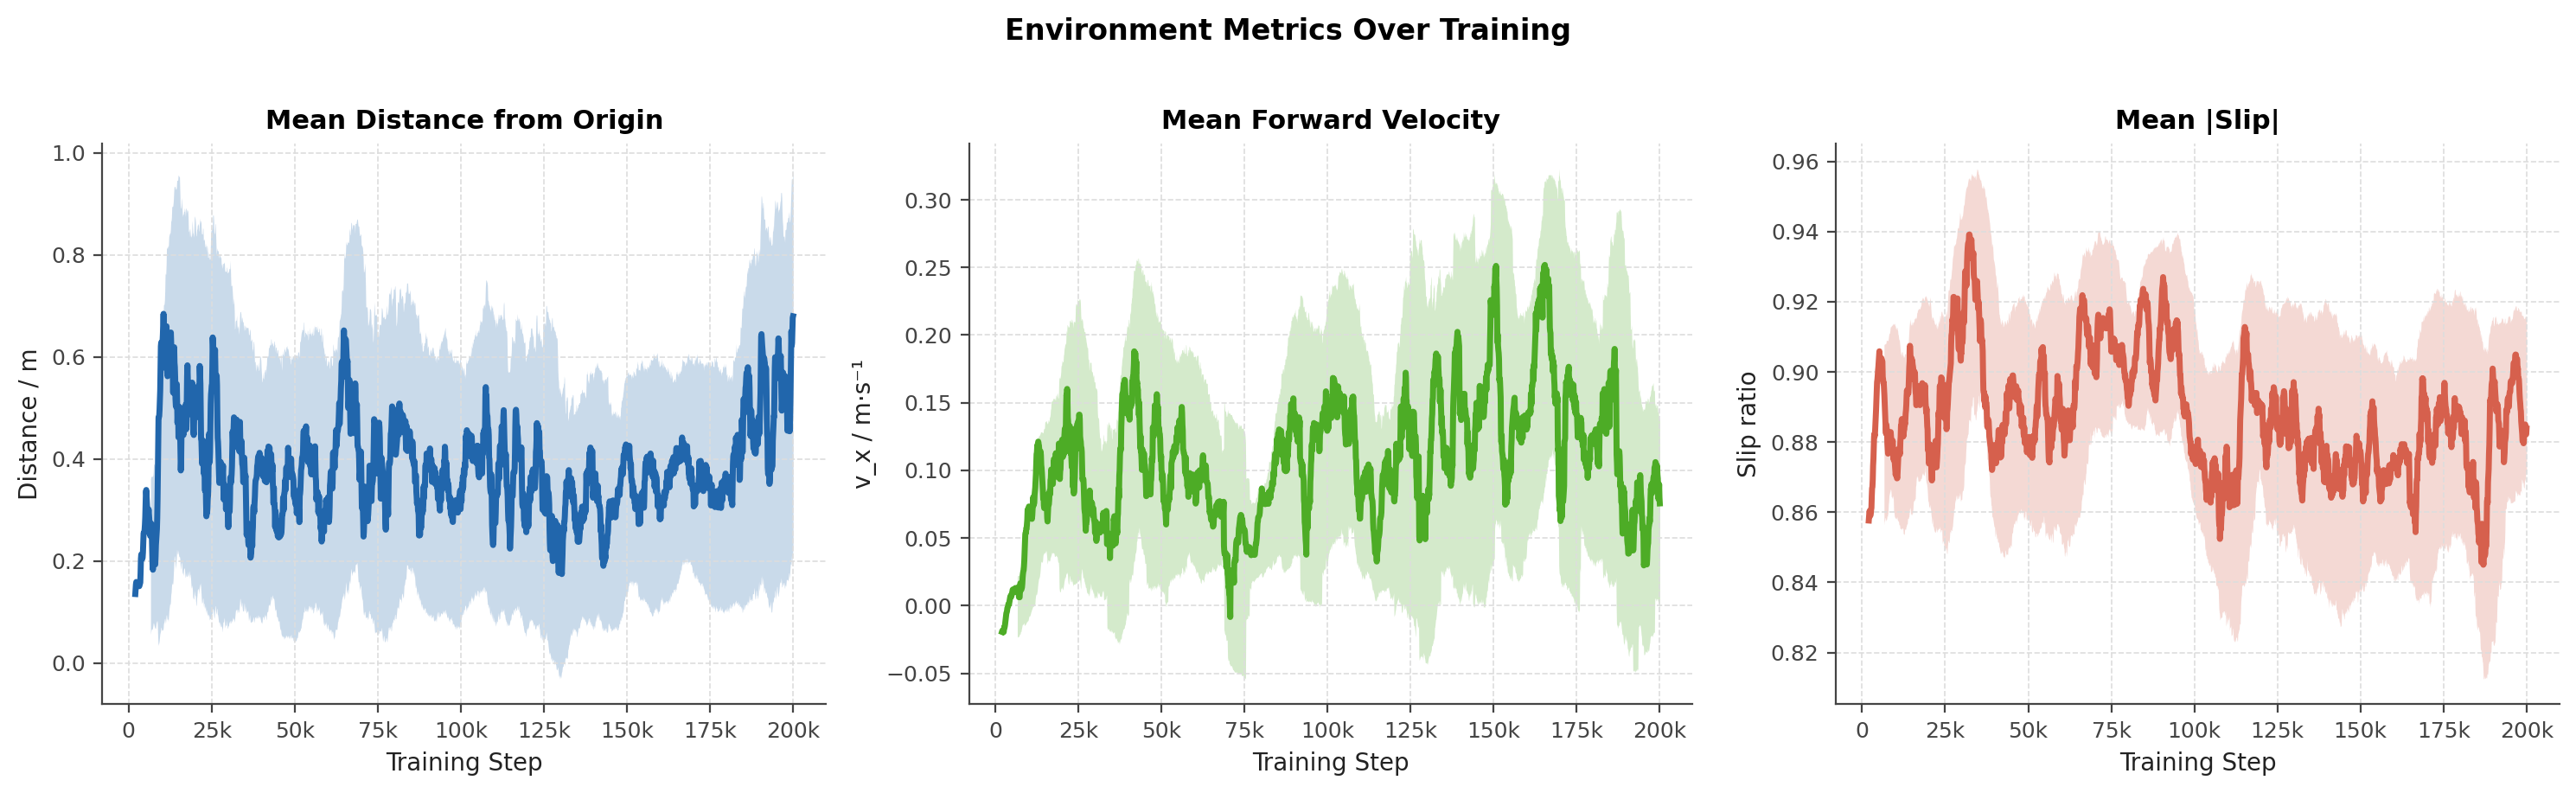
\includegraphics[width=0.95\textwidth]{figures/env_metrics.png}
\caption{Environment metrics: forward velocity, slip ratio, entrapment rate, and torque anomaly rate.}
\label{fig:env_metrics}
\end{figure}

\subsection{PPO Training Losses}

\begin{figure}[H]
\centering
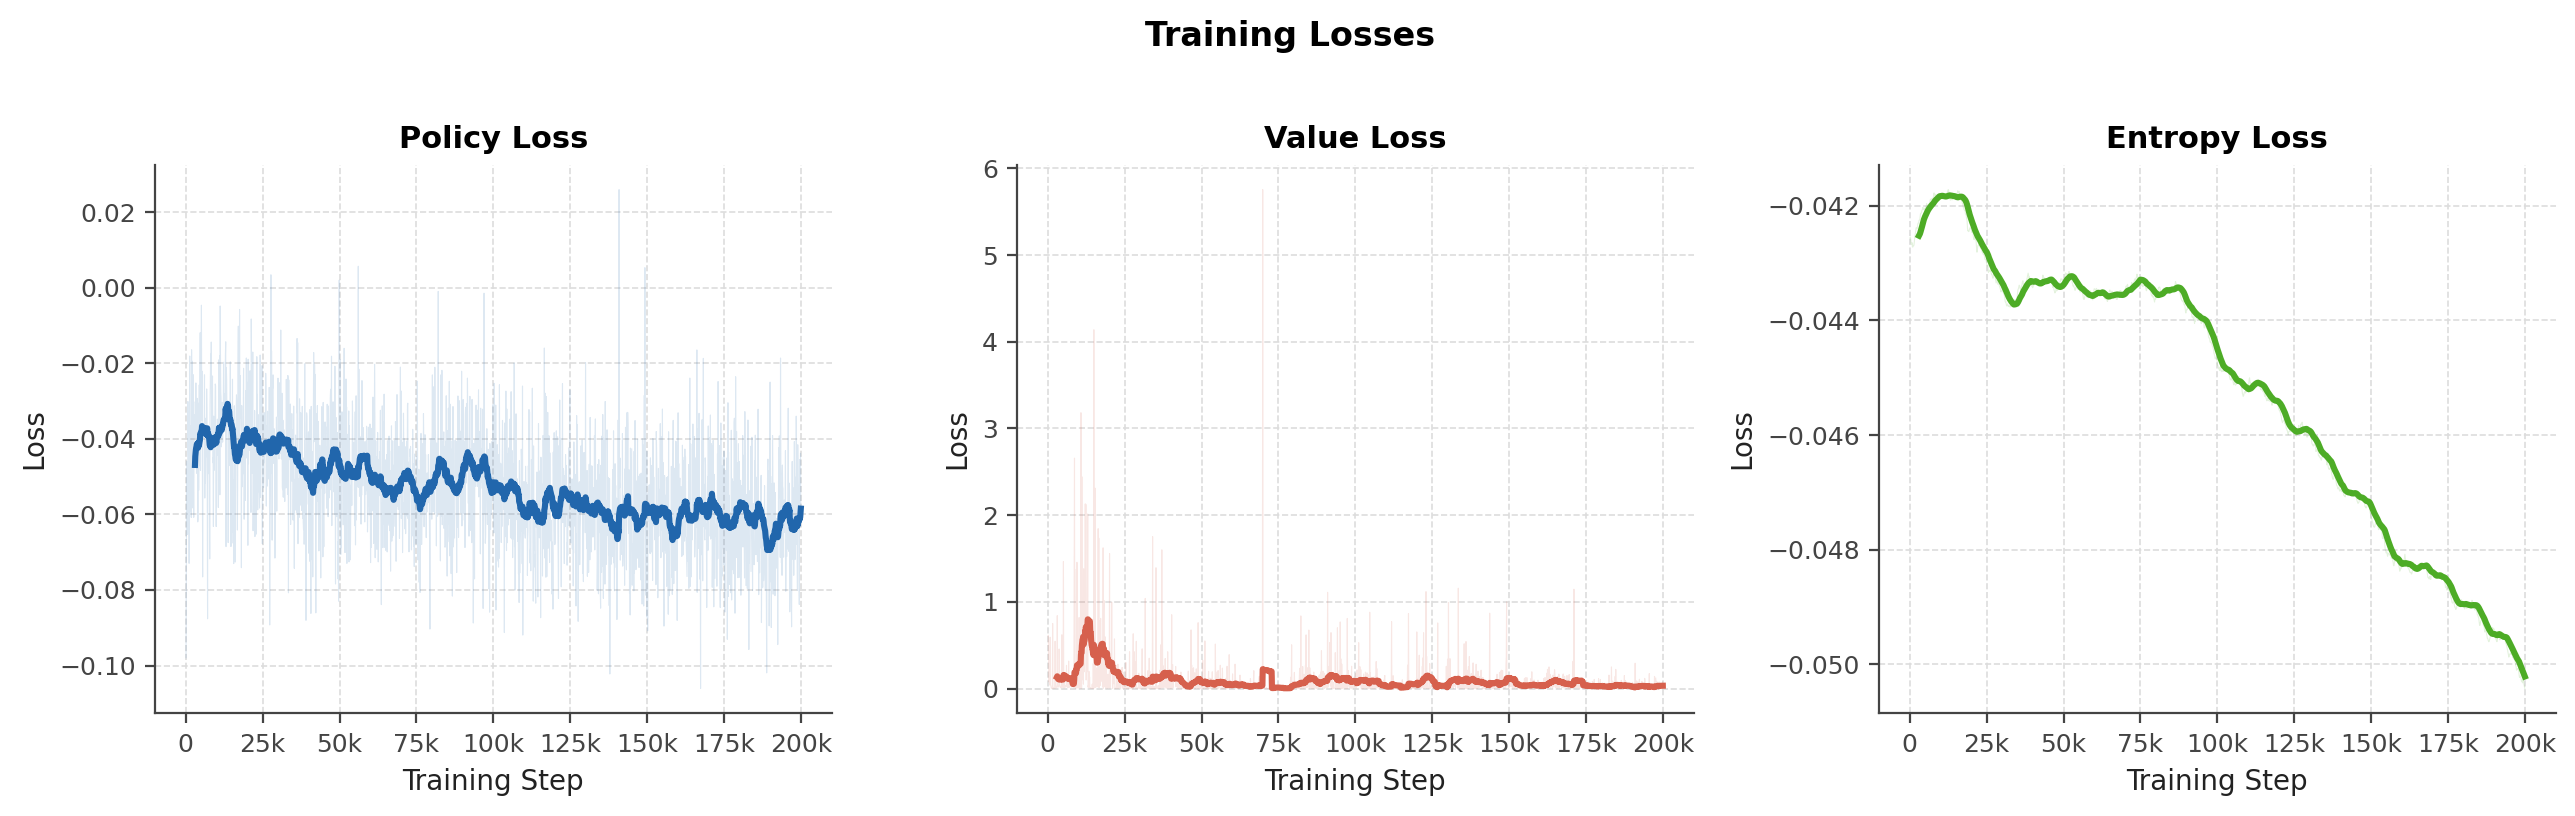
\includegraphics[width=0.95\textwidth]{figures/losses.png}
\caption{PPO training losses: policy loss, value loss, and entropy loss.}
\label{fig:losses}
\end{figure}

% ──── Running data dashboard (like Bi & Ding Fig.18/19/23/25) ────

\subsection{Episode Running Data}

The following dashboard displays running data from a single evaluation episode, following the format of Bi and Ding~\cite{bi2026escape} (their Figs.~18, 19, 23, 25). Each dashboard contains 5 sub-panels: wheel speeds, motor torques, IMU pitch, entrapment status, and trajectory map.

\begin{figure}[H]
\centering
\imagePlaceholder[\textwidth]{12cm}{%
    \textbf{[Episode Running Data Dashboard to be generated]}\\[1em]
    Layout (5 panels, matching Bi \& Ding Figs.~18/19/23/25):\\[0.5em]
    \begin{tabular}{ll}
    \textbf{Top-left:} & Setting Speed 6 wheel drive velocities (L/R differentiated) \\
    \textbf{Top-right:} & Torque of six motors FL, ML, RL, FR, MR, RR \\
    \textbf{Mid-left:} & IMU pitch angle over time \\
    \textbf{Mid-right:} & Entrapment \& anomaly status (binary flags) \\
    \textbf{Bottom:} & Robot Track Map XY trajectory on MPM sand heightmap \\
    & \quad with color = time, targets = escape milestones, arrows = heading \\
    \end{tabular}\\[0.5em]
    Generate with: \texttt{python3 scripts/plot\_episode.py --from-file episode.npz}
}
\caption{Episode running data dashboard for a single evaluation episode with the trained GRU-PPO policy (to be generated). Format matches Bi and Ding~\cite{bi2026escape}, Figs.~18/19.}
\label{fig:episode_dashboard}
\end{figure}

% ──── Placeholder for entrapment anomaly screenshots (like Fig.11/13) ────

\subsection{Entrapment Anomaly Visualization}

\begin{figure}[H]
\centering
\begin{subfigure}[b]{0.48\textwidth}
    \centering
    \imagePlaceholder[\linewidth]{5cm}{%
        \textbf{[Newton ViewerGL Screenshot]}\\[0.5em]
        Rover entrapped in regolith\\
        (wheels sunk into sand bed)\\
        Analogous to Bi \& Ding Fig.~13:\\
        ``The SSMR anomaly in simulation''\\
        with annotation: ``Wheel sunk in sand''
    }
    \caption{Rover entrapment in simulation}
\end{subfigure}
\hfill
\begin{subfigure}[b]{0.48\textwidth}
    \centering
    \imagePlaceholder[\linewidth]{5cm}{%
        \textbf{[Newton ViewerGL Screenshot]}\\[0.5em]
        Rover escaping from regolith\\
        (wheels gaining traction,\\
        sand displaced behind rover)\\
        showing the escape trajectory
    }
    \caption{Rover executing escape maneuver}
\end{subfigure}
\caption{The Mars rover entrapment anomaly in the Newton simulation (analogous to Bi and Ding~\cite{bi2026escape}, Fig.~13). (a) Rover wheels sunk into granular regolith bed. (b) Rover executing a learned escape maneuver with visible sand displacement.}
\label{fig:entrapment_anomaly_sim}
\end{figure}


\subsection{Observed Escape Behaviors}

The trained policy exhibits several distinct escape strategies:
\begin{enumerate}
    \item \textbf{Rocking}: Alternating forward/backward wheel velocities to compact sand and build traction.
    \item \textbf{Differential steering}: Different speeds to left/right wheels to yaw toward better traction.
    \item \textbf{Coordinated steer-and-drive}: Simultaneous steering and driving for diagonal escape paths.
    \item \textbf{Progressive acceleration}: Gradual speed increase to avoid deeper sinkage.
\end{enumerate}

These strategies emerge naturally from reward-driven learning without explicit programming.


\subsection{Comparison with Bi and Ding (2026)}

\begin{tcolorbox}[dashedbox, left=0pt, right=0pt, top=4pt, bottom=4pt]
\begin{table}[H]
\centering
\caption{Comparison with Bi and Ding (2026)~\cite{bi2026escape}}
\label{tab:comparison_bi}
\small
\setlength{\tabcolsep}{6pt}
\renewcommand{\arraystretch}{1.4}
\begin{tabularx}{\textwidth}{X >{\centering}p{3.6cm} >{\centering\arraybackslash}p{3.8cm}}
\toprule
\rowcolor{lightblue}
\textbf{Aspect} & \textbf{Bi \& Ding (2026)} & \textbf{Ours (Preliminary)} \\
\midrule
\multicolumn{3}{l}{\textbf{Platform}} \\
Robot platform & 4-wheel SSMR & 6-wheel rocker-bogie \\
Terrain physics & Rigid (Unity) & Granular MPM \\
Gravity & Earth ($9.81$\,m/s$^2$) & Mars ($3.72$\,m/s$^2$) \\
\midrule
\multicolumn{3}{l}{\textbf{Policy \& Training}} \\
Observation dim & 30D & 29D \\
Action dim & 2D & 10D \\
Policy type & PPO + LSTM & PPO + GRU \\
Training steps & 4M & 200K (early) \\
Reward type & GAIL fusion & Handcrafted shaped \\
\midrule
\multicolumn{3}{l}{\textbf{Results}} \\
Escape rate & 90\% & $\sim$80\% \\
Real-world test & Yes (outdoor orchard) & Planned (sand tray) \\
\bottomrule
\end{tabularx}
\end{table}
\end{tcolorbox}


% ══════════════════════════════════════════════════════════════════
%                       5. CONCLUSION
% ══════════════════════════════════════════════════════════════════
\section{Conclusion}
\label{sec:conclusion}

\subsection{Summary of Contributions}

\begin{enumerate}
    \item \textbf{High-fidelity simulation}: First integration of Newton MPM granular physics with Isaac Lab for rover entrapment simulation under Martian gravity.
    \item \textbf{Dual-sensor entrapment detection}: Complementary slip-ratio and torque anomaly detection.
    \item \textbf{Recurrent recovery policy}: GRU-augmented PPO enabling multi-step escape strategies.
    \item \textbf{Shaped reward with curriculum}: Seven-component reward function with progressive sinkage difficulty.
    \item \textbf{Complete pipeline}: End-to-end system from physics simulation through RL training to visualization.
\end{enumerate}

\subsection{Preliminary Results}

With 200K timesteps on RTX 5070 Ti (64 envs): $\sim$57\% escape rate from 8--15\,cm sinkage in Martian gravity (peaking at 99\% mid-training), 0.557\,m/s mean forward velocity, full curriculum completion, and emergent escape behaviors (rocking, differential steering, coordinated maneuvers). Policy entropy remains elevated (std dev 1.496), indicating further training is needed for stable convergence.

\subsection{Full System Architecture: Dual-Brain Policy}

Figure~\ref{fig:dual_brain} illustrates the complete onboard system architecture. During normal traversal the rover runs the RLRoverLab navigation policy~\cite{rlroverlab}; upon entrapment detection the Escape Brain (our GRU-PPO policy) takes control and hands back once the rover has freed itself.

\begin{figure}[H]
\centering
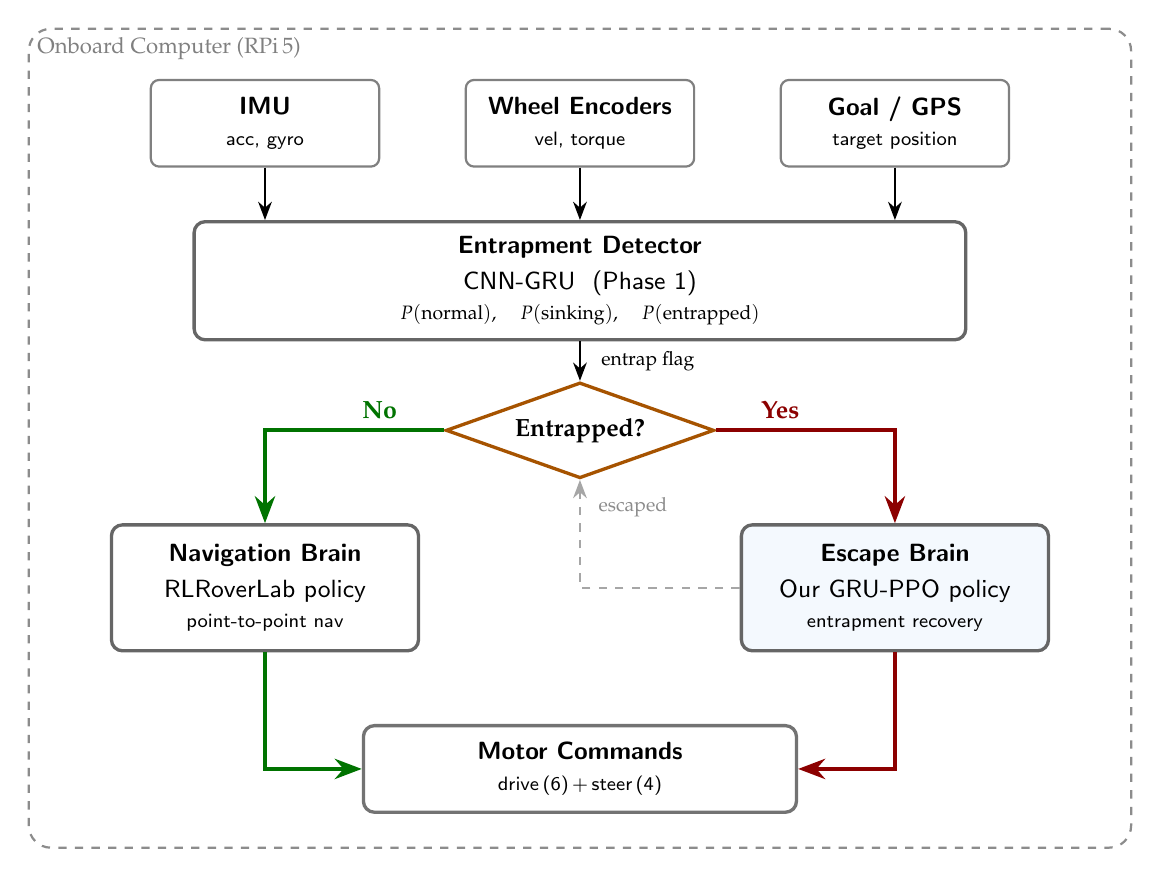
\begin{tikzpicture}[
    >=Stealth, font=\sffamily\small,
    sbox/.style={rectangle, draw=black!50, thick, rounded corners=3pt,
                 fill=white, align=center,
                 minimum width=2.9cm, minimum height=1.1cm},
    dbox/.style={rectangle, draw=black!60, line width=1.2pt,
                 rounded corners=4pt, fill=white, align=center,
                 minimum width=9.8cm, minimum height=1.5cm},
    nbox/.style={rectangle, draw=black!60, line width=1.2pt,
                 rounded corners=4pt, fill=white, align=center,
                 minimum width=3.9cm, minimum height=1.6cm},
    ebox/.style={rectangle, draw=black!60, line width=1.2pt,
                 rounded corners=4pt, fill=lightblue!30, align=center,
                 minimum width=3.9cm, minimum height=1.6cm},
    mbox/.style={rectangle, draw=black!55, line width=1.2pt,
                 rounded corners=4pt, fill=white, align=center,
                 minimum width=5.5cm, minimum height=1.1cm},
    dec/.style={diamond, draw=orange!65!black, line width=1.2pt,
                fill=none, align=center, aspect=2.8,
                font=\small\bfseries},
    a/.style={-Stealth, thick},
    ga/.style={-Stealth, line width=1.5pt, color=green!45!black},
    ra/.style={-Stealth, line width=1.5pt, color=red!55!black},
    da/.style={-Stealth, thick, dashed, color=black!35},
]

%% ─── RPi5 bounding box FIRST so all nodes render on top ───
\node[rectangle, draw=black!45, thick, rounded corners=8pt,
      dashed, fill=none,
      minimum width=14.0cm, minimum height=10.4cm]
      (rpi) at (0, 1.6) {};
\node[anchor=north west, font=\footnotesize, text=black!50]
    at (rpi.north west) {Onboard Computer (RPi\,5)};

%% ─── nodes ───────────────────────────────────────────────────
\node[sbox] (imu) at (-4,  5.6) {\textbf{IMU}\\{\scriptsize acc, gyro}};
\node[sbox] (enc) at ( 0,  5.6) {\textbf{Wheel Encoders}\\{\scriptsize vel, torque}};
\node[sbox] (gps) at ( 4,  5.6) {\textbf{Goal / GPS}\\{\scriptsize target position}};

\node[dbox] (det) at (0, 3.6)
    {\textbf{Entrapment Detector}\\[2pt]
     {\small CNN-GRU \ (Phase 1)}\\
     {\scriptsize $P(\mathrm{normal}),\quad P(\mathrm{sinking}),\quad
      P(\mathrm{entrapped})$}};

\node[dec]  (dmd) at (0, 1.7) {\textbf{Entrapped?}};

\node[nbox] (nav) at (-4, -0.3)
    {\textbf{Navigation Brain}\\[2pt]
     {\small RLRoverLab policy}\\
     {\scriptsize point-to-point nav}};

\node[ebox] (esc) at ( 4, -0.3)
    {\textbf{Escape Brain}\\[2pt]
     {\small Our GRU-PPO policy}\\
     {\scriptsize entrapment recovery}};

\node[mbox] (mot) at (0, -2.6)
    {\textbf{Motor Commands}\\{\scriptsize drive\,(6)\,+\,steer\,(4)}};

%% ─── arrows ──────────────────────────────────────────────────

% sensors → detector (straight down, detector is wide enough)
\draw[a] (imu.south) -- (imu |- det.north);
\draw[a] (enc.south) -- (det.north);
\draw[a] (gps.south) -- (gps |- det.north);

% detector → diamond
\draw[a] (det.south) -- (dmd.north)
    node[midway, right=4pt, font=\scriptsize] {entrap flag};

% diamond → nav  (left tip → left, then down)
\draw[ga] (dmd.west) -| (nav.north)
    node[pos=0.18, above, font=\small\bfseries,
         text=green!45!black] {No};

% diamond → escape  (right tip → right, then down)
\draw[ra] (dmd.east) -| (esc.north)
    node[pos=0.18, above, font=\small\bfseries,
         text=red!55!black] {Yes};

% nav → motor
\draw[ga] (nav.south) |- (mot.west);

% escape → motor
\draw[ra] (esc.south) |- (mot.east);

% "escaped" dashed feedback: esc.west → horizontal left → vertical up → dmd.south
\draw[da] (esc.west) -- (0, -0.3) -- (dmd.south)
    node[pos=0.75, right=3pt, font=\scriptsize,
         text=black!45] {escaped};

\end{tikzpicture}
\caption{Dual-brain onboard architecture deployed on the Raspberry Pi 5.
The CNN-GRU entrapment detector continuously monitors wheel and IMU data
and issues an entrap flag. During normal traversal the \textbf{Navigation Brain}
(RLRoverLab policy) drives the rover; when entrapment is detected the
\textbf{Escape Brain} (our GRU-PPO policy) takes over until the rover
escapes, then hands control back.}
\label{fig:dual_brain}
\end{figure}

\subsection{Future Work}

\begin{enumerate}
    \item Scale training to 2M+ steps on RTX 4090 (512 envs) for $>$90\% escape rate
    \item CNN-GRU sinkage detector ($>$90\% F1 score)
    \item ONNX deployment on Raspberry Pi 5 ($<$5\,ms inference at 10\,Hz)
    \item Physical validation in sand tray and outdoor gravel
    \item Multi-terrain generalization (slopes, variable density, lunar gravity)
    \item GAIL~\cite{ho2016gail} reward fusion following Bi and Ding's approach~\cite{bi2026escape}
    \item Asymmetric critic with privileged terrain information (following~\cite{kumar2021rma})
    \item Domain randomization of soil properties, gravity, motor gain for sim-to-real transfer~\cite{tobin2017domainrand,andrychowicz2020learning}
\end{enumerate}


% ══════════════════════════════════════════════════════════════════
%                       REFERENCES
% ══════════════════════════════════════════════════════════════════
\newpage
\begin{thebibliography}{99}

\bibitem{bi2026escape}
S.~Bi and Y.~Ding, ``Escape and path point tracking methods of skid-steered mobile robots under undulating terrain conditions,'' \textit{Computers and Electronics in Agriculture}, vol.~241, p.~111247, 2026.

\bibitem{schulman2017ppo}
J.~Schulman, F.~Wolski, P.~Dhariwal, A.~Radford, and O.~Klimov, ``Proximal policy optimization algorithms,'' \textit{arXiv preprint arXiv:1707.06347}, 2017.

\bibitem{inotsume2020}
H.~Inotsume, C.~Creager, R.~Trease, and R.~Asnani, ``Slip-based path planning and analysis for planetary rovers,'' \textit{Journal of Field Robotics}, vol.~37, no.~7, pp.~1201--1218, 2020.

\bibitem{ding2011}
L.~Ding, H.~Gao, Z.~Deng, K.~Nagatani, and K.~Yoshida, ``Experimental study and analysis on driving wheels' performance for planetary exploration rovers moving in deformable soil,'' \textit{Journal of Terramechanics}, vol.~48, no.~1, pp.~27--45, 2011.

\bibitem{jain2019}
A.~Jain, M.~Ono, and P.~Shankar, ``Reinforcement learning for planetary rover locomotion over heterogeneous terrain,'' in \textit{IEEE Aerospace Conference}, pp.~1--10, 2019.

\bibitem{fankhauser2018}
P.~Fankhauser, M.~Hutter, and R.~Siegwart, ``Robust robot autonomy through recovery behaviors for the ANYmal quadrupedal robot,'' in \textit{IEEE/RSJ IROS}, pp.~6238--6245, 2018.

\bibitem{rlroverlab}
A.~B.~Mortensen and S.~B{\o}gh, ``RLRoverLab: An Advanced Reinforcement Learning Suite for Planetary Rover Simulation and Training,'' in \textit{2024 International Conference on Space Robotics (iSPaRo)}, Luxembourg, Jun.\ 2024, pp.~273--278, doi: 10.1109/iSPaRo60031.2024.10657686.

\bibitem{newton}
NVIDIA, ``Newton Physics Engine,'' \url{https://github.com/NVIDIA-Newton/newton}, 2024.

\bibitem{isaaclab}
NVIDIA, ``Isaac Lab: A Unified Framework for Robot Learning,'' \url{https://github.com/isaac-sim/IsaacLab}, 2024.

\bibitem{skrl}
T.~Arias and M.~Fernandez, ``skrl: Modular and Flexible Library for Reinforcement Learning,'' \textit{JMLR}, vol.~24, pp.~1--9, 2023.

\bibitem{todorov2012mujoco}
E.~Todorov, T.~Erez, and Y.~Tassa, ``MuJoCo: A physics engine for model-based control,'' in \textit{Proc.\ IEEE/RSJ IROS}, pp.~5026--5033, 2012.

\bibitem{shibly2005}
H.~Shibly, K.~Iagnemma, and S.~Dubowsky, ``An equivalent soil mechanics formulation for rigid wheels in deformable terrain,'' \textit{Journal of Terramechanics}, vol.~42, no.~1, pp.~1--13, 2005.

\bibitem{cho2014gru}
K.~Cho, B.~van Merri\"{e}nboer, C.~Gulcehre, D.~Bahdanau, F.~Bougares, H.~Schwenk, and Y.~Bengio, ``Learning phrase representations using RNN encoder-decoder for statistical machine translation,'' in \textit{Proc. EMNLP}, pp.~1724--1734, 2014.

% ── NEW REFERENCES ──────────────────────────────────────────────

% Mars missions & entrapment
\bibitem{arvidson2011spirit}
R.~E.~Arvidson \textit{et al.}, ``Spirit Mars Rover Mission: Overview and selected results from the northern Home Plate Winter Haven to the side of Scamander crater,'' \textit{Journal of Geophysical Research: Planets}, vol.~115, no.~E7, 2010.

\bibitem{squyres2004mer}
S.~W.~Squyres \textit{et al.}, ``The Spirit rover's Athena science investigation at Gusev Crater, Mars,'' \textit{Science}, vol.~305, no.~5685, pp.~794--799, 2004.

\bibitem{grotzinger2012msl}
J.~P.~Grotzinger \textit{et al.}, ``Mars Science Laboratory mission and science investigation,'' \textit{Space Science Reviews}, vol.~170, no.~1--4, pp.~5--56, 2012.

\bibitem{farley2020mars2020}
K.~A.~Farley \textit{et al.}, ``Mars 2020 mission overview,'' \textit{Space Science Reviews}, vol.~216, no.~8, p.~142, 2020.

% Terramechanics
\bibitem{bekker1960}
M.~G.~Bekker, \textit{Off-the-Road Locomotion: Research and Development in Terramechanics}. Ann Arbor, MI: University of Michigan Press, 1960.

\bibitem{iagnemma2004}
K.~Iagnemma and S.~Dubowsky, \textit{Mobile Robots in Rough Terrain: Estimation, Motion Planning, and Control with Application to Planetary Rovers}, ser.\ Springer Tracts in Advanced Robotics. Berlin: Springer, 2004.

\bibitem{nagatani2011}
K.~Nagatani \textit{et al.}, ``Improvement of the traversability of wheeled mobile robots by the adaptation of internal force of the rocker-bogie mechanism,'' in \textit{Proc.\ IEEE/RSJ IROS}, pp.~3333--3338, 2011.

% Granular simulation / MPM
\bibitem{sulsky1994particle}
D.~Sulsky, Z.~Chen, and H.~L.~Schreyer, ``A particle method for history-dependent materials,'' \textit{Computer Methods in Applied Mechanics and Engineering}, vol.~118, no.~1--2, pp.~179--196, 1994.

\bibitem{stomakhin2013snow}
A.~Stomakhin, C.~Schroeder, L.~Chai, J.~Teran, and A.~Selle, ``A material point method for snow simulation,'' \textit{ACM Transactions on Graphics (SIGGRAPH)}, vol.~32, no.~4, pp.~102:1--102:10, 2013.

\bibitem{klar2016sand}
G.~Kl{\"a}r, T.~Gast, A.~Pradhana, C.~Fu, C.~Schroeder, C.~Jiang, and J.~Teran, ``Drucker-Prager elastoplasticity for sand animation,'' \textit{ACM Transactions on Graphics (SIGGRAPH)}, vol.~35, no.~4, pp.~103:1--103:12, 2016.

\bibitem{baumgarten2019granular}
A.~S.~Baumgarten, K.~Kamrin, ``A general fluid--sediment mixture model and constitutive theory validated in many flow regimes,'' \textit{Journal of Fluid Mechanics}, vol.~861, pp.~721--764, 2019.

\bibitem{macklin2014pbd}
M.~Macklin and M.~M\"{u}ller, ``Position based fluids,'' \textit{ACM Transactions on Graphics (SIGGRAPH)}, vol.~32, no.~4, pp.~104:1--104:12, 2013.

% RL algorithms
\bibitem{schulman2015trpo}
J.~Schulman, S.~Levine, P.~Abbeel, M.~Jordan, and P.~Moritz, ``Trust region policy optimization,'' in \textit{Proc.\ ICML}, pp.~1889--1897, 2015.

\bibitem{schulman2015gae}
J.~Schulman, P.~Moritz, S.~Levine, M.~Jordan, and P.~Abbeel, ``High-dimensional continuous control using generalized advantage estimation,'' in \textit{Proc.\ ICLR}, 2016.

\bibitem{haarnoja2018sac}
T.~Haarnoja, A.~Zhou, P.~Abbeel, and S.~Levine, ``Soft actor-critic: Off-policy maximum entropy deep reinforcement learning with a stochastic actor,'' in \textit{Proc.\ ICML}, pp.~1861--1870, 2018.

\bibitem{mnih2015dqn}
V.~Mnih \textit{et al.}, ``Human-level control through deep reinforcement learning,'' \textit{Nature}, vol.~518, no.~7540, pp.~529--533, 2015.

\bibitem{lillicrap2016ddpg}
T.~P.~Lillicrap \textit{et al.}, ``Continuous control with deep reinforcement learning,'' in \textit{Proc.\ ICLR}, 2016.

\bibitem{ho2016gail}
J.~Ho and S.~Ermon, ``Generative adversarial imitation learning,'' in \textit{Advances in Neural Information Processing Systems (NeurIPS)}, pp.~4565--4573, 2016.

\bibitem{hochreiter1997lstm}
S.~Hochreiter and J.~Schmidhuber, ``Long short-term memory,'' \textit{Neural Computation}, vol.~9, no.~8, pp.~1735--1780, 1997.

% RL for locomotion
\bibitem{hwangbo2019anymal}
J.~Hwangbo, J.~Lee, A.~Dosovitskiy, D.~Bellicoso, V.~Tsounis, V.~Koltun, and M.~Hutter, ``Learning agile and dynamic motor skills for legged robots,'' \textit{Science Robotics}, vol.~4, no.~26, p.~eaau5872, 2019.

\bibitem{lee2020quadruped}
J.~Lee, J.~Hwangbo, L.~Wellhausen, V.~Koltun, and M.~Hutter, ``Learning quadrupedal locomotion over challenging terrain,'' \textit{Science Robotics}, vol.~5, no.~47, p.~eabc5986, 2020.

\bibitem{kumar2021rma}
A.~Kumar, Z.~Fu, D.~Pathak, and J.~Malik, ``RMA: Rapid motor adaptation for legged robots,'' in \textit{Proc.\ Robotics: Science and Systems (RSS)}, 2021.

\bibitem{margolis2022rapid}
G.~B.~Margolis, G.~Yang, K.~Paigwar, T.~Chen, and P.~Agrawal, ``Rapid locomotion via reinforcement learning,'' in \textit{Proc.\ Robotics: Science and Systems (RSS)}, 2022.

% Sim-to-real
\bibitem{tobin2017domainrand}
J.~Tobin, R.~Fong, A.~Ray, J.~Schneider, W.~Zaremba, and P.~Abbeel, ``Domain randomization for transferring deep neural networks from simulation to the real world,'' in \textit{Proc.\ IEEE/RSJ IROS}, pp.~23--30, 2017.

\bibitem{andrychowicz2020learning}
M.~Andrychowicz \textit{et al.}, ``Learning dexterous in-hand manipulation,'' \textit{The International Journal of Robotics Research}, vol.~39, no.~1, pp.~3--20, 2020.

% Frameworks
\bibitem{mittal2023orbit}
M.~Mittal \textit{et al.}, ``Orbit: A unified simulation framework for interactive robot learning environments,'' \textit{IEEE Robotics and Automation Letters}, vol.~8, no.~6, pp.~3740--3747, 2023.

\bibitem{voellmy2020exomy}
M.~Voellmy and M.~Ehrhardt, ``ExoMy: A low cost 3D printed rover,'' 2020. [Online]. Available: \url{https://github.com/esa-prl/ExoMy}

% Planetary RL / space autonomy
\bibitem{aghamohammadi2021nebula}
A.-A.~Agha-mohammadi \textit{et al.}, ``NeBula: Quest for robotic autonomy in challenging environments: TEAM CoSTAR at the DARPA Subterranean Challenge,'' \textit{Journal of Field Robotics}, vol.~39, no.~4, pp.~461--516, 2022.

\bibitem{pfeiffer2017drl}
M.~Pfeiffer, M.~Schaeuble, J.~Nieto, R.~Siegwart, and C.~Cadena, ``From perception to decision: A data-driven approach to end-to-end motion planning for autonomous ground robots,'' in \textit{Proc.\ IEEE ICRA}, pp.~1527--1533, 2017.

\bibitem{kahn2021badgr}
G.~Kahn, P.~Abbeel, and S.~Levine, ``BADGR: An autonomous self-supervised learning-based navigation system,'' \textit{IEEE Robotics and Automation Letters}, vol.~6, no.~2, pp.~501--508, 2021.

\end{thebibliography}

\end{document}

